%\documentclass[a4paper,12pt]{book}
%\usepackage{multirow}
%\usepackage{fixltx2e}
%\usepackage{array}
%\usepackage[english]{babel}
%\usepackage{amsmath}
%\usepackage{todonotes}
%\usepackage[]{algorithm2e}
%\begin{document}

\chapter{Our Proposed Approaches}
\lhead{Chapter 3. \emph{Our Proposed Approaches}}

In this section, we will discuss our proposed approach for mining frequent pattern over large uncertain stream data. Stream Data has a special property that it comes and flows away. For this reason, we will always lose data after data stream has flown away. To resolve this, we will propose a window-batch based approach, where we will keep the most recent information in a tree structure because the most recent data is most valuable. Later we will show how the window will slide, remove old data and insert new data in the tree. As, for uncertain data stream each same item in the different transaction has different existential probability, it becomes very difficult to merge (share) these nodes in the tree. This uncertainty property of item makes the tree huge. We have proposed a new \emph{U\textsuperscript{cap}} value for each item that helps to share a single node when constructing the tree which we named as \emph{US-tree}. We will show that our proposed tree \emph{US-tree} will be very compact and very efficient for later mining. Later, we will describe an approach for mining the \emph {US-tree} named \emph{USFP-growth} which is \emph{FP-growth} like approach. Later we will propose a method for filtering and remove false positive from finding most probable candidate frequent patterns.

\section{Uncertain Stream Data Properties}
    In this chapter, we will talk about data properties. Our data has two special properties (1) Stream and (2) Uncertainty. For these properties, it becomes very much hard to get valuable and interesting information from data. So first we discuss the data set properties.

    \subsection{Stream Property}
    Stream data are such data those come and go away. They cannot be stored in any patterns. Data streams are continuous and unbounded. This property makes finding patterns so much difficult. As when stream flows away we lose them, we have no choice to store data and scan more than one time we have to find some technique to store valuable information that will help to find valuable information later. For example, table-\ref{table:uncertain_stream_transaction} shows the uncertain stream transaction database. Here \emph{T\textsubscript{1}, T\textsubscript{2}, T\textsubscript{3}, T\textsubscript{4}, T\textsubscript{5}, T\textsubscript{6}, T\textsubscript{7}, T\textsubscript{8}, T\textsubscript{9}} comes one after another and goes away. It may occur that when \emph{T\textsubscript{10}} comes after a long time of \emph{T\textsubscript{4} or T\textsubscript{5} or T\textsubscript{6}} came. So there is no way get \emph{T\textsubscript{4}} when \emph{T\textsubscript{10}} comes. As we are always interested in most recent data, because most recent data are most valuable, we proposed a sliding window based approach that holds the most recent data in our proposed \emph{US-tree} to hold valuable meta information for further valuable frequent pattern extraction.

    \subsection{Uncertainty Property}
    Data is not always precise. Hardware limitations, loss of information during transmission, sampling errors etc. can make precise data uncertain. For this reason the data existence is not for sure. Each time data can comes with a probability value that is called its existential probability. For example, in table-\ref{table:uncertain_stream_transaction}  we can see each transaction having items with item's probability. This value is its existential probability. Let for transaction-\emph{T\textsubscript{2}} there is four items \emph{a(0.9), c(0.6), d(0.5)} and \emph{e(0.2)}. Here \emph{0.9, 0.6, 0.5, 0.2} all are existential probability of corresponding \emph{a, c, d, e}. That means \emph{a's} existential probability is \emph{0.9}. Probability of existence of \emph{a} in those transactions is \emph{0.9}. This property makes mining very much difficult. This property says that in different transaction in a transaction data base same item can have different existential probability. So finding similarity between same items becomes another matter to worry about. For expected support calculation of item becomes very much tough. For expected support calculation equation-\ref{equation:exp_sup} is used.
    %\documentclass{article}
%\usepackage{fixltx2e}
%\begin{document}
\begin{equation}\label{equation:exp_sup}
\emph ExpSup \qquad = \qquad \sum_{i = 0}^{UDB} [\prod_{x \in I } p(x , t_i)]
\end{equation}
\begin{center}


\textbf{\emph {where,}}\\ 
\begin{itemize}
\item
\textbf{\emph {I}} is itemset,
\item
\textbf{\emph { p(x, ti)}} is existential probability value for any item \textbf{\emph {x}} in transaction \textbf{\emph {t\textsubscript{i}}} 
\item
\textbf{\emph {UDB}} is an uncertain database.

\end{itemize}
\end{center}
%
%\end{document}
    From this equation we can see that calculation of support is not that easy and straight forward like certain data. Certain data support is calculated just counting the total existence of that items in the transaction were as for uncertain data it depends on its existential probability. It may occur that some data set exists many times in a transaction database but with a low probability, so ultimately the data must not be frequent. For example, if we want to find the support of \emph{ae} of table-\ref{table:uncertain_stream_transaction} then we need to do the following calculation. For \emph{T\textsubscript{2}} $0.9*0.2=0.18$, \emph{T\textsubscript{2}} $0.9*0.1=0.09$, \emph{T\textsubscript{3}} $0.0$, \emph{T\textsubscript{4}} $0.0$, \emph{T\textsubscript{5}} $0.0$, \emph{T\textsubscript{6}} $0.9*0.3=0.27$, \emph{T\textsubscript{7}} $0.1*0.2=0.02$, \emph{T\textsubscript{8}}=$0.0$ and \emph{T\textsubscript{9}}=$0.0$.$Sup_{ae} =Sup_{ae(T_1)}+Sup_{ae(T_2)}+Sup_{ae(T_3)}+Sup_{ae(T_4)}+Sup_{ae(T_5)}+Sup_{ae(T_6)}+Sup_{ae(T_7)}+Sup_{ae(T_8)}+Sup_{ae(T_9)}=0.18+0.09+0.0+0.0+0.0+0.27+0.0+0.02+0.0+0.0=0.54$ So if \emph{minimum support is $0.9$} than \emph{ae} is not frequent but \emph{ae} exists four times in the transaction. So it makes very much difficult to find which a pattern is important or not.
    
    
\section{Preliminaries}
    \paragraph{Definition-1 : Uncertain Frequent Pattern} 
    Given DB = \emph{\{T\textsubscript{1}, T\textsubscript{2}, T\textsubscript{3} . . . T\textsubscript{N} \}} , an uncertain database with \emph{N} transactions where minimum expected support threshold is $\delta$. The problem is to mine frequent item-sets \emph{FI} $\subset$ DB, where $ExpSup(FI_i) \geq \delta $ and $FI_i \in FI$.
    
    \paragraph{Definition-2 : Batch} 
    A group of consecutive transactions from a transaction \emph{DB}inserted in \emph{US-tree} at a time. Let table-\ref{table:uncertain_stream_transaction} batch size = \emph{3}. \emph{T\textsubscript{1}, T\textsubscript{2}, T\textsubscript{3}} is one batch and its batch-1. Then next three \emph{T\textsubscript{4}, T\textsubscript{5}, T\textsubscript{6}} is one batch and its batch-2.
    
    \paragraph{Definition-3 : Window} Window is the size of batch consecutive one \emph{US-tree} can hold. Let table-\ref{table:transaction_batch} be an example of grouped transaction and batch number tagged. So for window size \emph{2} The in a certain time batch-1 and batch-2 will create a window. Then after some times when batch-3 comes then batch-2 and batch-3 will create the next window.
    
    \paragraph{Definition-4 : U\textsuperscript{cap}} 
    The following equation is for \emph{U\textsuperscript{cap}}    calculation.
    %\documentclass{article}
%\usepackage{amsmath}
%\begin{document}
\begin{equation}\label{equation:cap}
\text{\emph{U\textsuperscript{cap}}}(X_r) =\begin{cases}
				P(X_1), & \text{if $ h = 1$}\\
				P(X_r)*M, & \text{if $ h > 1$}
             
\end{cases}
where, M=max_{1\leq q\leq h}P(X_q)
\end{equation}
%\end{document}
    For transaction \emph{DB} example in table-\ref{table:uncertain_stream_transaction} for \emph{T\textsubscript{1}}, \emph{U\textsuperscript{cap}} of \emph{a{0.9}} is $0.9$ as a is the first item. For \emph{c(0.6)} \emph{U\textsuperscript{cap}} is $0.9*0.6=0.45$, \emph{d(0.50)} \emph{U\textsuperscript{cap}} is $0.9*0.5=0.45$ and \emph{e(0.2)} \emph{U\textsuperscript{cap}} is $0.9*0.2=0.18$. \emph{U\textsuperscript{cap}} is the upper bound of existential probability. As we are taking the max of all previous items coming in a particular order all items or item sets having existential probability must be less than or equal \emph{U\textsuperscript{cap}}. that is $\forall(i,j)\{ P(I_i)*P(I_j)\leq U_{cap}(I_j)\}$ where $i < j$. So support must be less than or equal \emph{U\textsubscript{cap}}.\\
    Calculated \emph{U\textsuperscript{cap}} should be the upper bound of two item's existential probability because we have taken the maximum value of item that has come earlier. So, by two item set support that can have maximum support value, is \emph{U\textsuperscript{cap}} value. Item set having \emph{U\textsuperscript{cap}} less than minimum support must frequent. Though this may cause some false positives but it is for sure that no false negative will insert into this. 
    %\documentclass{article} 
%\usepackage{graphicx}  
%\usepackage{multirow}
%\usepackage[table]{xcolor}
%\usepackage{fixltx2e}
%\usepackage{array}
%
%\begin{document}
\begin{table}[t]
\centering

\begin{tabular}{|c|c|c|c|c|c|}
\hline
& No & \multicolumn{4}{c|}{Items in Transaction} \\ \hline \hline
\multirow{3}{*}{Batch 1}	&	T\textsubscript{1} & a(0.9) & c(0.6) & d(0.5) & e(0.2)\\
							&	T\textsubscript{2} & a(0.9) & b(0.4) & e(0.1) & --    \\
							&	T\textsubscript{3} & a(0.2) & c(0.9) & d(0.7) & --    \\\hline
\multirow{3}{*}{Batch 2}	&	T\textsubscript{4} & b(0.3) & c(0.9) & -- & --\\
							&	T\textsubscript{5} & a(0.1) & b(0.3) & c(0.9) & --    \\
							&	T\textsubscript{6} & a(0.9) & e(0.3) & -- & --        \\\hline
\multirow{3}{*}{Batch 3}	&	T\textsubscript{7} & a(0.1) & d(0.6) & e(0.2) & --    \\
							&	T\textsubscript{8} & a(0.1) & c(0.2) & f(0.6) & --    \\
							&	T\textsubscript{9} & c(0.2) & d(0.9) & f(0.6) & --    \\\hline
							
\multirow{3}{*}{Batch 4}	&	T\textsubscript{10} &  --  &  --  &  --  & --    \\
							&	T\textsubscript{11} &  --  &  --  &  --  & --    \\
							&	T\textsubscript{12} &  --  &  --  &  --  & --    \\\hline
\end{tabular}
\caption{Uncertain Stream Transaction Data Divided into Batch}
\label{table:transaction_batch}
\end{table}


%
%\end{document}
    \paragraph{Definition-5 : False Positive}
    \paragraph{Definition-5 : False Negatives}
    
\section{Mining Frequent Patterns from Uncertain Databases}
    Our proposed algorithm is divided into five parts. (1) Grouping transactions into batches and window and giving each item in a transaction a prefix value is called \emph{U\textsuperscript{cap}}. (2) Insert transaction into \emph {US-tree}. (3) Sliding the \emph {US-tree} (4) mining the \emph {US-tree} with \emph{USFP-growth} algorithm and (5) Eliminating false positive (not frequent but exists infrequent item set) . For simulating our approach we consider Table~\ref{table:uncertain_stream_transaction} as uncertain stream transaction data. For this simulation, we consider window size as 2 and batch size 3. That means 3 transactions creates a batch and 2 batches create a window. After completing window construction (inserting batch 1 and 2), the \emph {US-tree} will be full. When new batch comes we slide the window. That means we remove oldest batch batch-1 and put batch-2 as the old batch. Then insert new batch in the tree as batch-3. So for window size 2 the tree always contains at most 2 batches. Thus, the tree always holds the latest information. In next subsections, we will elaborately explain our approach of every step.

    \subsection{Preparation}
    %\documentclass{article} 
%\usepackage{graphicx}  
%\usepackage{multirow}
%\usepackage[table]{xcolor}
%\usepackage{fixltx2e}
%\usepackage{array}
%
%\begin{document}
\begin{table}
\centering

\begin{tabular}{|l|l|l|l|l|l|}
\hline
	Batch No& No & \multicolumn{4}{c|}{Items in Transaction} \\ \hline \hline
	\multirow{3}{*}{Batch 1}	&	T\textsubscript{1} & a(0.9) & c(0.54) & d(0.45) & e(0.18)			\\\cline{2-6}
								&	T\textsubscript{2} & a(0.9) & b(0.36) & e(0.09) & --			\\\cline{2-6}
								&	T\textsubscript{3} & a(0.2) & c(0.18) & d(0.63) & --			\\\hline
	\multirow{3}{*}{Batch 2}	&	T\textsubscript{4} & b(0.3) & c(0.27) & 	--     & --	\\\cline{2-6}
								&	T\textsubscript{5} & a(0.1) & b(0.03) & c(0.27) & --  			\\\cline{2-6}
								&	T\textsubscript{6} & a(0.9) & e(0.27) & --	   & --  			\\\hline
	\multirow{3}{*}{Batch 3}	&	T\textsubscript{7} & a(0.1) & d(0.06) & e(0.12) & --	\\\cline{2-6}
								&	T\textsubscript{8} & a(0.1) & c(0.02) & f(0.12) & --   			\\\cline{2-6}
								&	T\textsubscript{9} & c(0.2) & d(0.09) & f(0.54) & --   			\\\hline
								
	\multirow{3}{*}{Batch 4}	&	T\textsubscript{10} &  --  &  --  &  --  & --    				\\\cline{2-6}
								&	T\textsubscript{11} &  --  &  --  &  --  & --    				\\\cline{2-6}
								&	T\textsubscript{12} &  --  &  --  &  --  & --    				\\\hline
	\end{tabular}
\caption{Window and Batch of Table\ref{table:uncertain_stream_transaction}}
\label{table:prefix_assigned}
\end{table}


%
%\end{document}
    In this section we will describe the batch and window grouping and the prefix value \emph{U\textsuperscript{cap}} calculation. First we calculate batch and window calculation and grouping our transaction data. As we describe earlier for the example Table-\ref{table:uncertain_stream_transaction} easy simulation we take batch size as \emph{$3$} and window size as \emph{$2$}. So first \emph{$3$} transactions \emph{T\textsubscript{1}}, \emph{T\textsubscript{2}} and \emph{T\textsubscript{3}} are grouped and labeled as \emph{Batch-1}. Then next \emph{$3$} \emph{T\textsubscript{4}}, \emph{T\textsubscript{5}} and \emph{T\textsubscript{6}} are grouped together and labeled as \emph{Batch-2}. Next \emph{$3$} \emph{T\textsubscript{7}}, \emph{T\textsubscript{8}} and \emph{T\textsubscript{9}} are grouped together and labeled as \emph{Batch-3}. Thus the consecutive next \emph{$3$} transaction should be grouped as batch and ready to be inserted into \emph{US-tree}. As our window size is $2$, after inserting two batches into the \emph{US-tree} the window will be completed. Before inserting next batch \emph{Batch-3} we need to remove \emph{Batch-1}(oldest one) from tree and move \emph{Batch-2} to \emph{Batch-1 's} position and then insert new batch, \emph{Batch-3}. Thus the latest information is inserted and kept into the \emph{US-tree}. table-\ref{table:transaction_batch} shows the window and batch grouped for stream transaction example table-\ref{table:uncertain_stream_transaction}.
    For this calculation we earlier proposed an equation-\ref{equation:cap}. From this equation we can create \emph{U\textsuperscript{cap}} for each item in a transaction. To calculate one transaction, for each item in a transaction, if item is the first item in a transaction than item's existential probability is its \emph{U\textsuperscript{cap}} value, otherwise item's \emph{U\textsuperscript{cap}} is max of previous items existential probability multiplied by item's  own existential probability. For example, let Table-\ref{table:transaction_batch} T1 is \emph{a(0.9), c(0.6), d(0.5), e(0.2)}. \\
    In this transaction item \emph{a(0.9)} is the first item. So its \emph{U\textsuperscript{cap}} is 0.9.\\
    For second item, \emph{c(0.60)} previous item is only \emph{a(0.90)}. So c's $\emph{U\textsuperscript{cap}} = 0.9*0.6 = 0.54$. \\
    For third item, \emph{d(0.50)} there are two items before it, \emph{a(0.9)} and \emph{c(0.6)}. Among them \emph{a} has max existential probability, that is \emph{0.9}. So \emph{d's } $\emph{U\textsuperscript{cap}} = 0.9*0.5 = 0.45$.\\
    For fourth item \emph{e(0.2)} there are three items before it, \emph{a(0.9)} ,\emph{c(0.6)} and \emph{d(0.5)}. Among them \emph{a} has max existential probability is \emph{0.9}. So \emph{e's}  $\emph{U\textsuperscript{cap}} = 0.9*0.2 = 0.45$. Thus we can calculate each item's \emph{U\textsuperscript{cap}} value for a transaction. For easier understanding we have calculated all the item's \emph{U\textsuperscript{cap}} of Table-\ref{table:transaction_batch} and put into Table-\ref{table:prefix_assigned}.
    
    
    
    \subsection{US-tree Construction}
    In this section we will describe about our tree construction \emph{US-tree}. We have described earlier about our batch and window. A batch should be inserted into the tree in its own window slot. After inserting all batches, the window will be complete and be ready to mine. We said earlier section that our tree will be very compact. For this we have proposed an approach for sharing nodes. For sharing same tree nodes two items with same id and order should not care about own existential probability. If item is already in the tree with same id then two items should share the node. Thus the tree will be very compact. When inserting an item in the tree the \emph{U\textsuperscript{cap}} of the tree should be updated by adding the prefix value of the node. Thus each batch should be inserted into the tree. The algorithm is given in the algorithm section Algorithm-\ref{algorithm:tree_construction}.
    %\documentclass{article}
%\usepackage{graphicx}
%\usepackage{caption}
%\usepackage{subcaption}
%
%\begin{document}
\begin{figure}[!tbp]
  \centering
	\fbox{  
	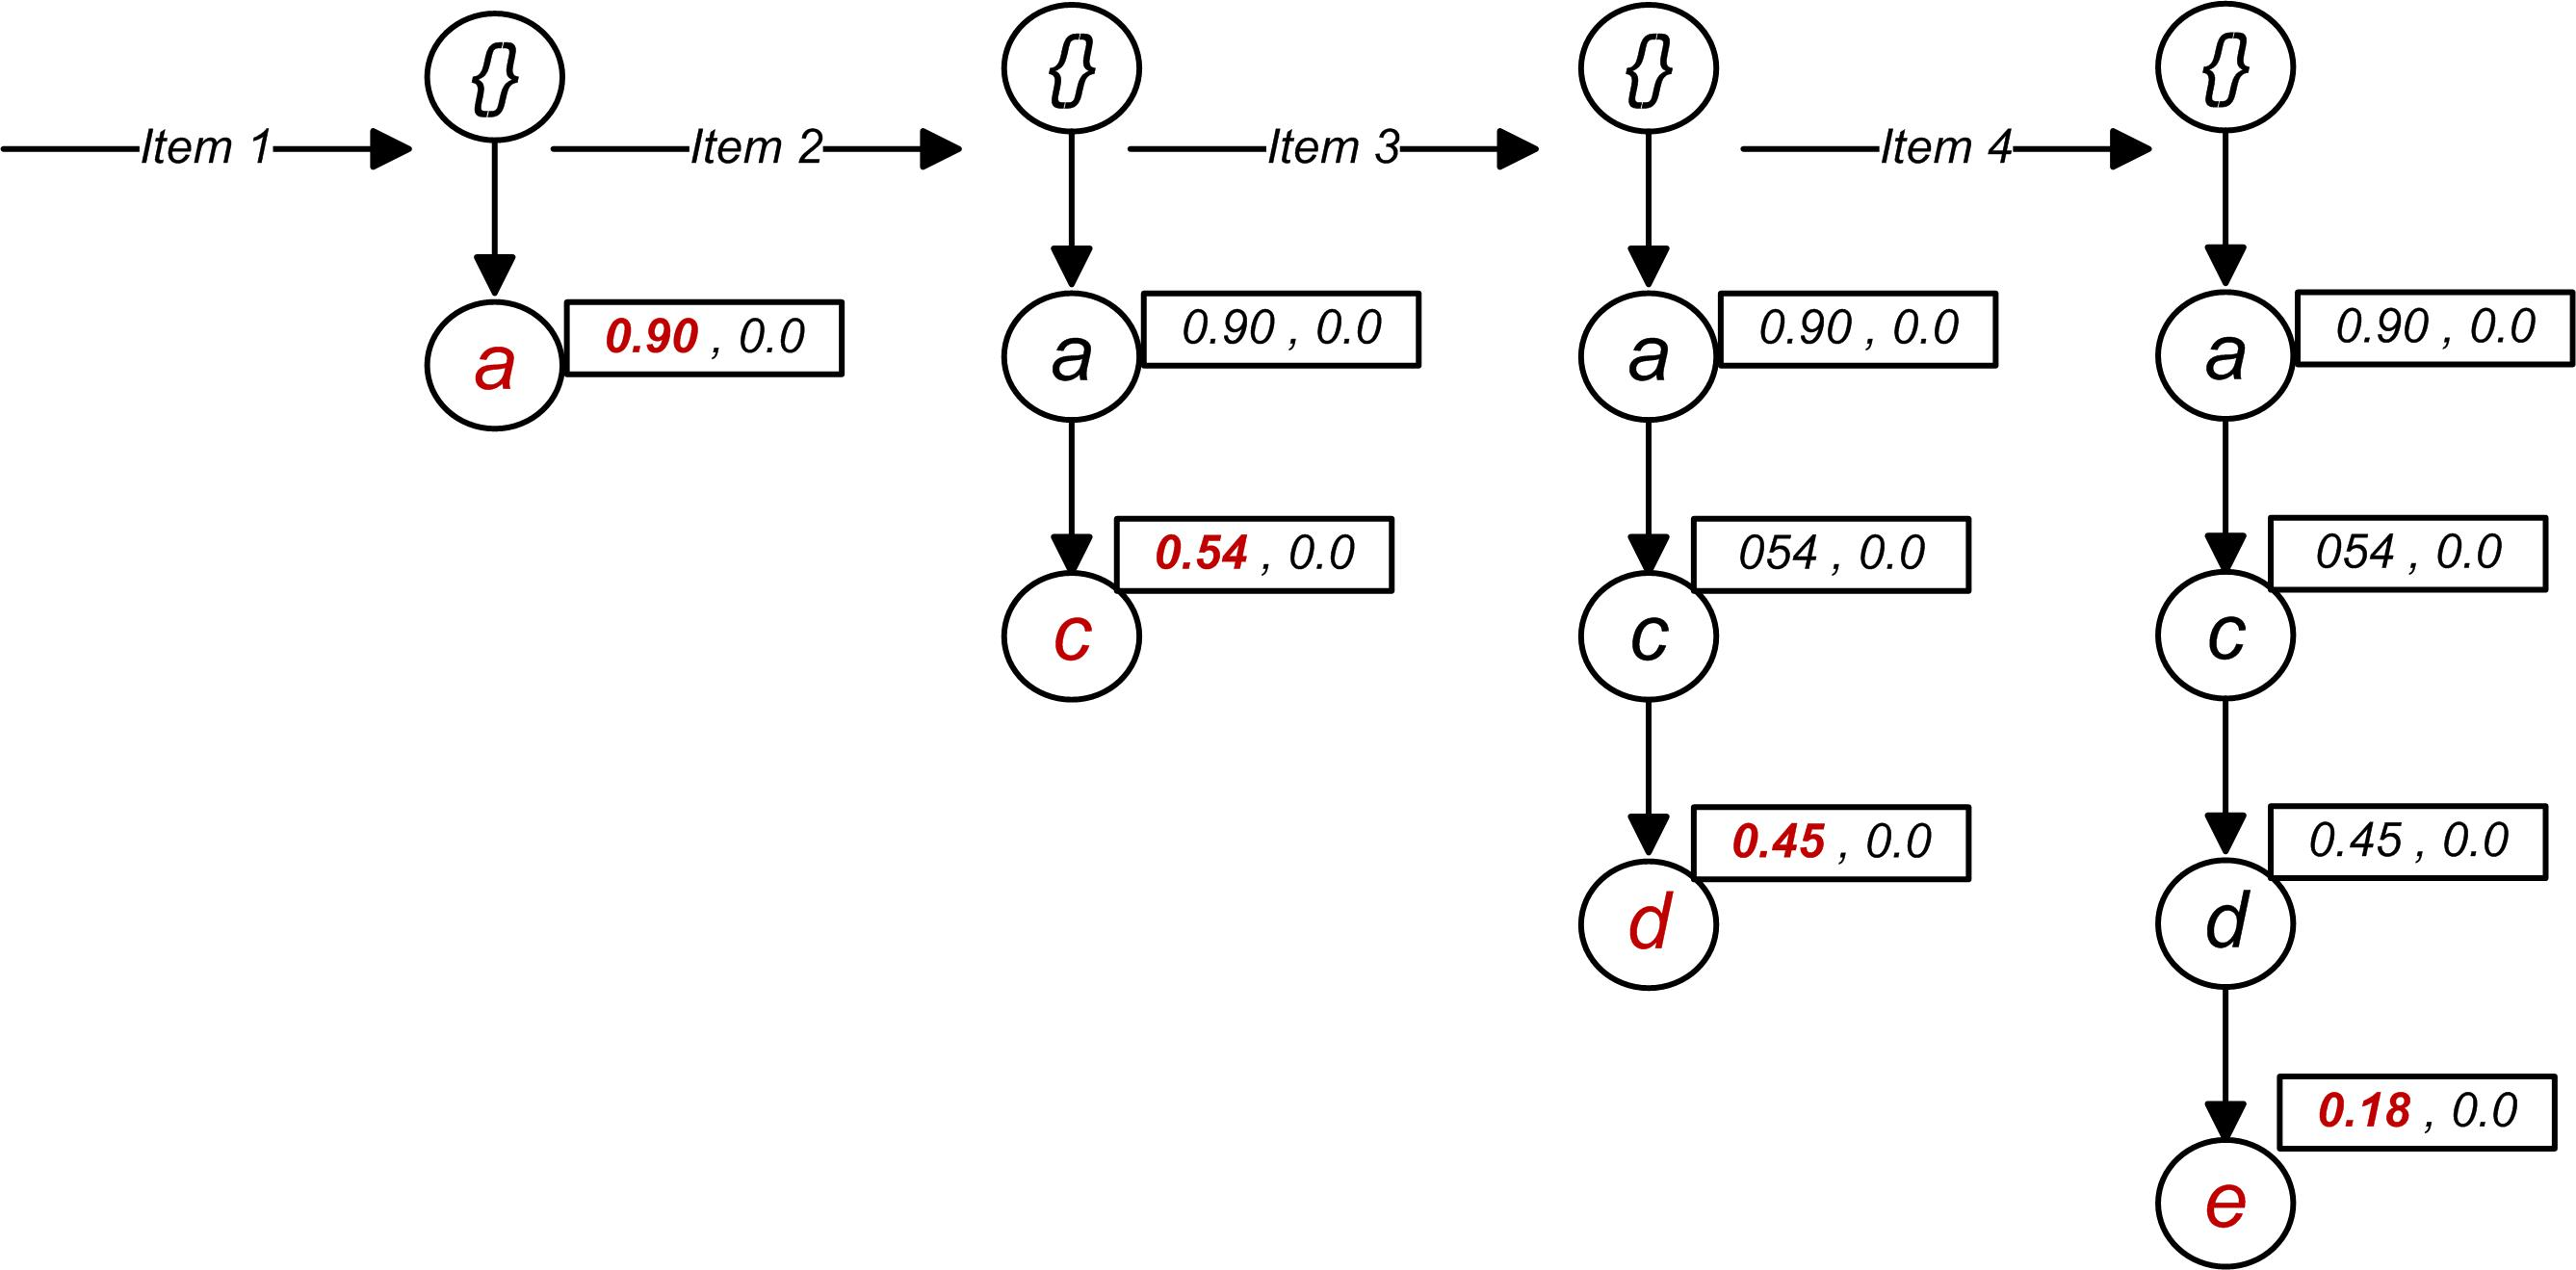
\includegraphics[width=.8\textwidth,height=5cm]{images/sim_01.jpg}  
	}
	\caption{Inserting \emph{T\textsubscript{1}} into \emph{US-tree}}
	\label{figure:t1}
\end{figure}
\begin{frame}

\begin{figure}[!tbp]
  \centering
	\fbox{  
	 	\begin{subfigure}[b]{0.40\textwidth}
	 	\centering
	    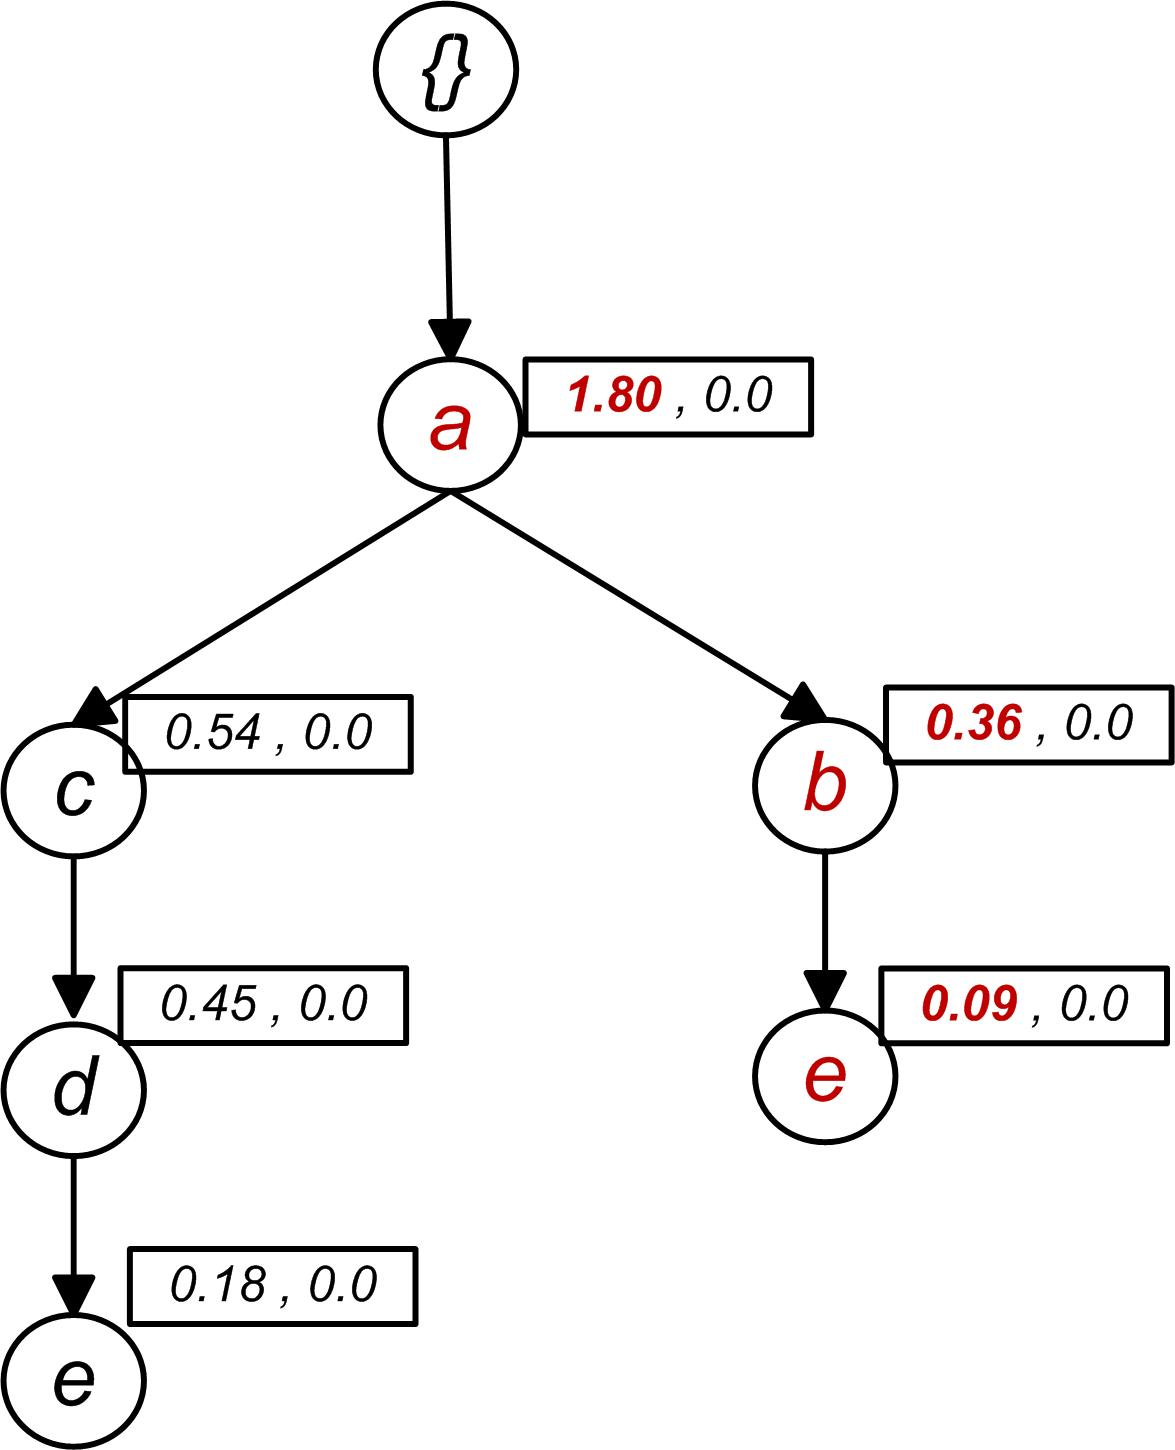
\includegraphics[width=.8\textwidth,height=4cm]{images/sim_02.jpg}
	    \caption{T\textsubscript{2}}
		\end{subfigure}
	  
	 	\begin{subfigure}[b]{0.40\textwidth}
	 	\centering
	    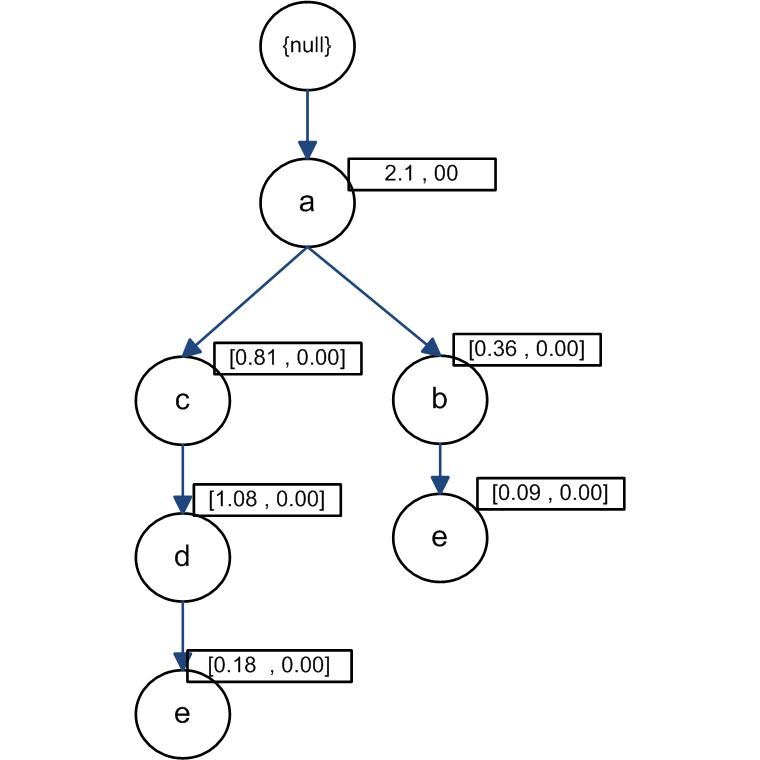
\includegraphics[width=.8\textwidth,height=4cm]{images/sim_03.jpg}
	    \caption{T\textsubscript{3}}
		\end{subfigure}
	}
 \caption{Inserting \emph{T\textsubscript{2}} and \emph{T\textsubscript{3}} in \emph{US-tree}}
 \label{figure:t23}
\end{figure}
\end{frame}
\begin{frame}

\begin{figure}[!tbp]
  \centering
	\fbox{  
	 	\begin{subfigure}[b]{0.22\textwidth}
	 	\centering
	    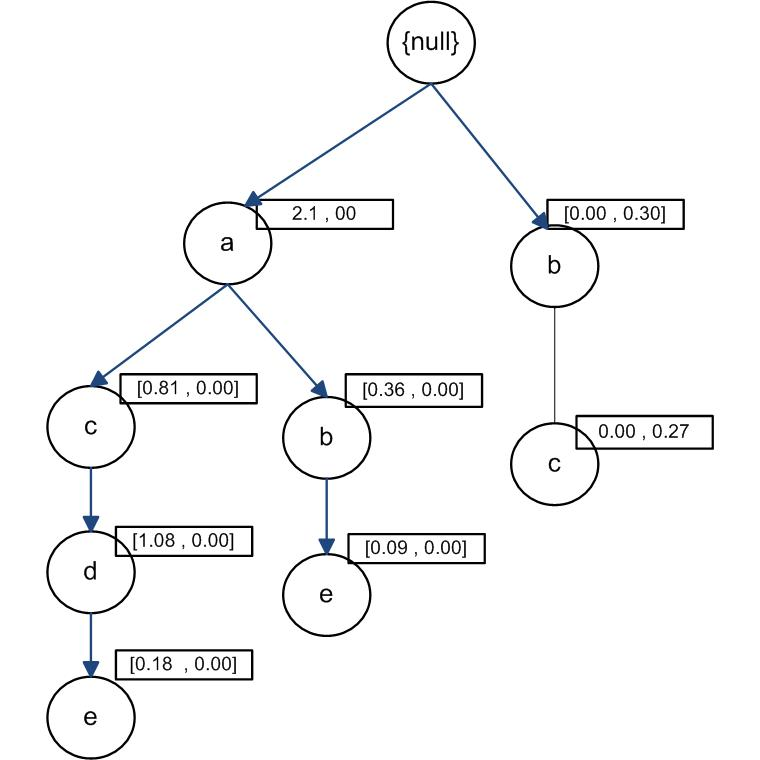
\includegraphics[width=\textwidth,height=4.0cm]{images/sim_04.jpg}
	    \caption{T\textsubscript{4}}
		\end{subfigure}
	 
	 	\begin{subfigure}[b]{0.27\textwidth}
	 	\centering
	    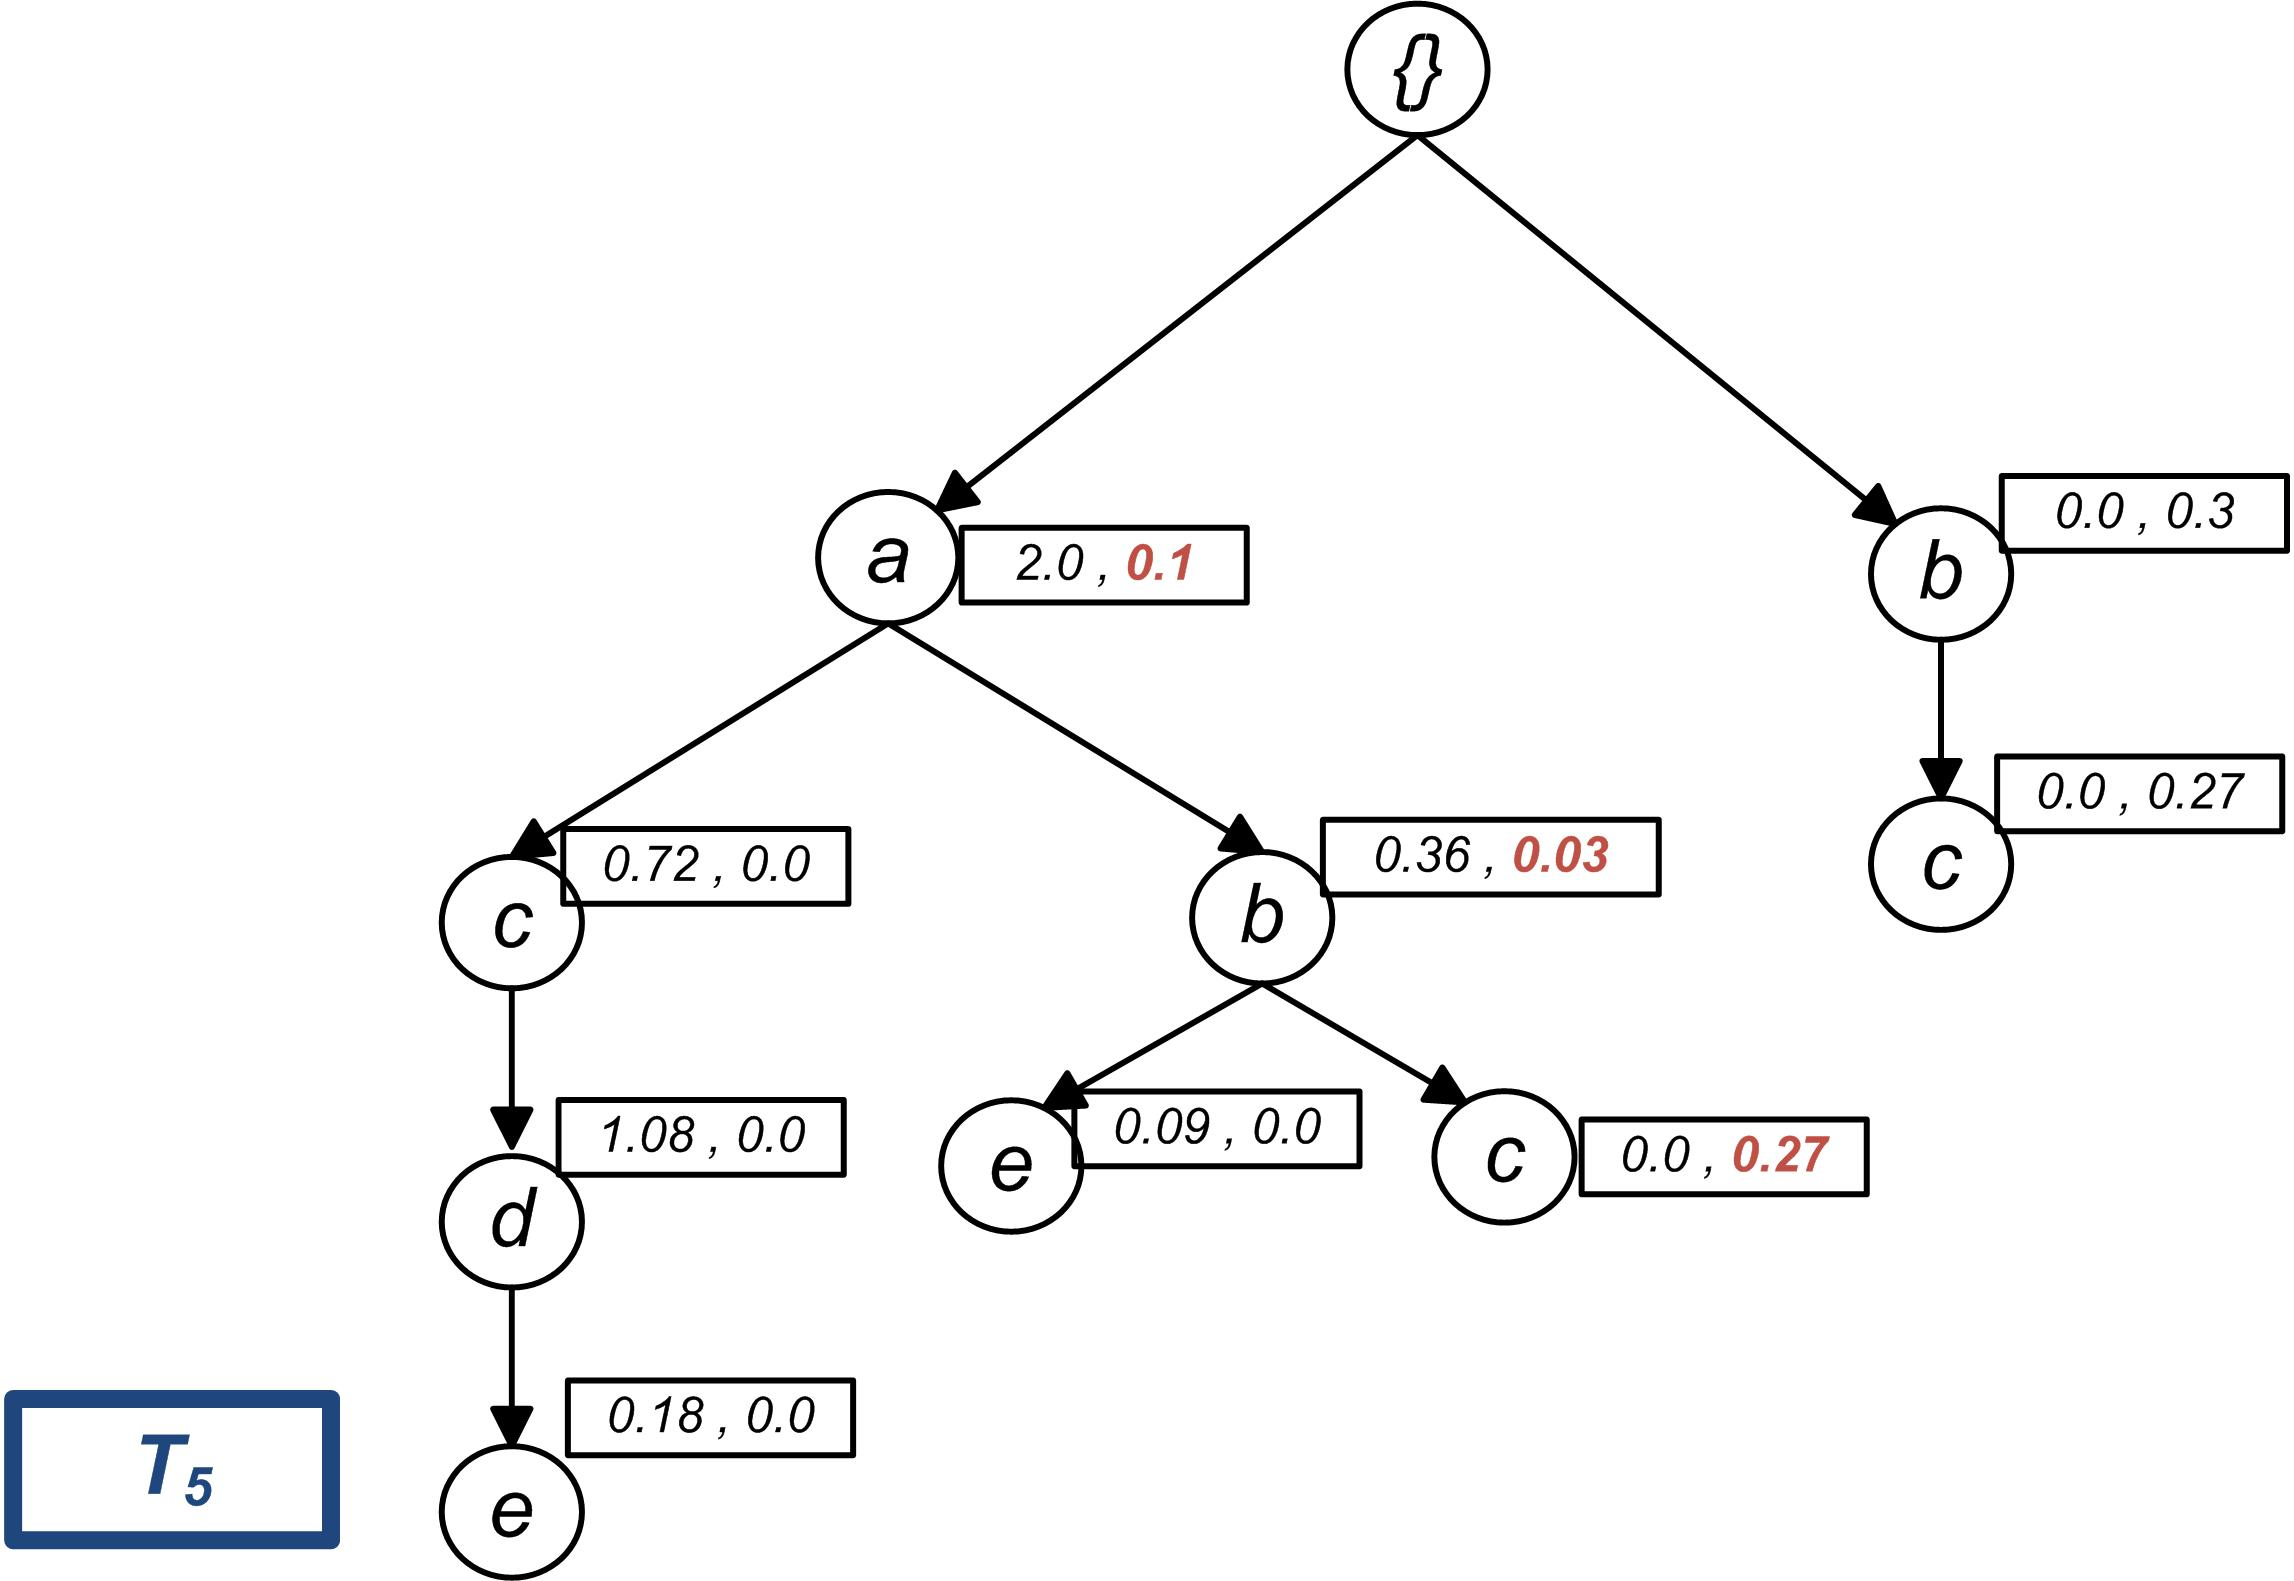
\includegraphics[width=\textwidth,height=4.0cm]{images/sim_05.jpg}
	    \caption{T\textsubscript{5}}
		\end{subfigure}
	  
	 	\begin{subfigure}[b]{0.31\textwidth}
	 	\centering
	    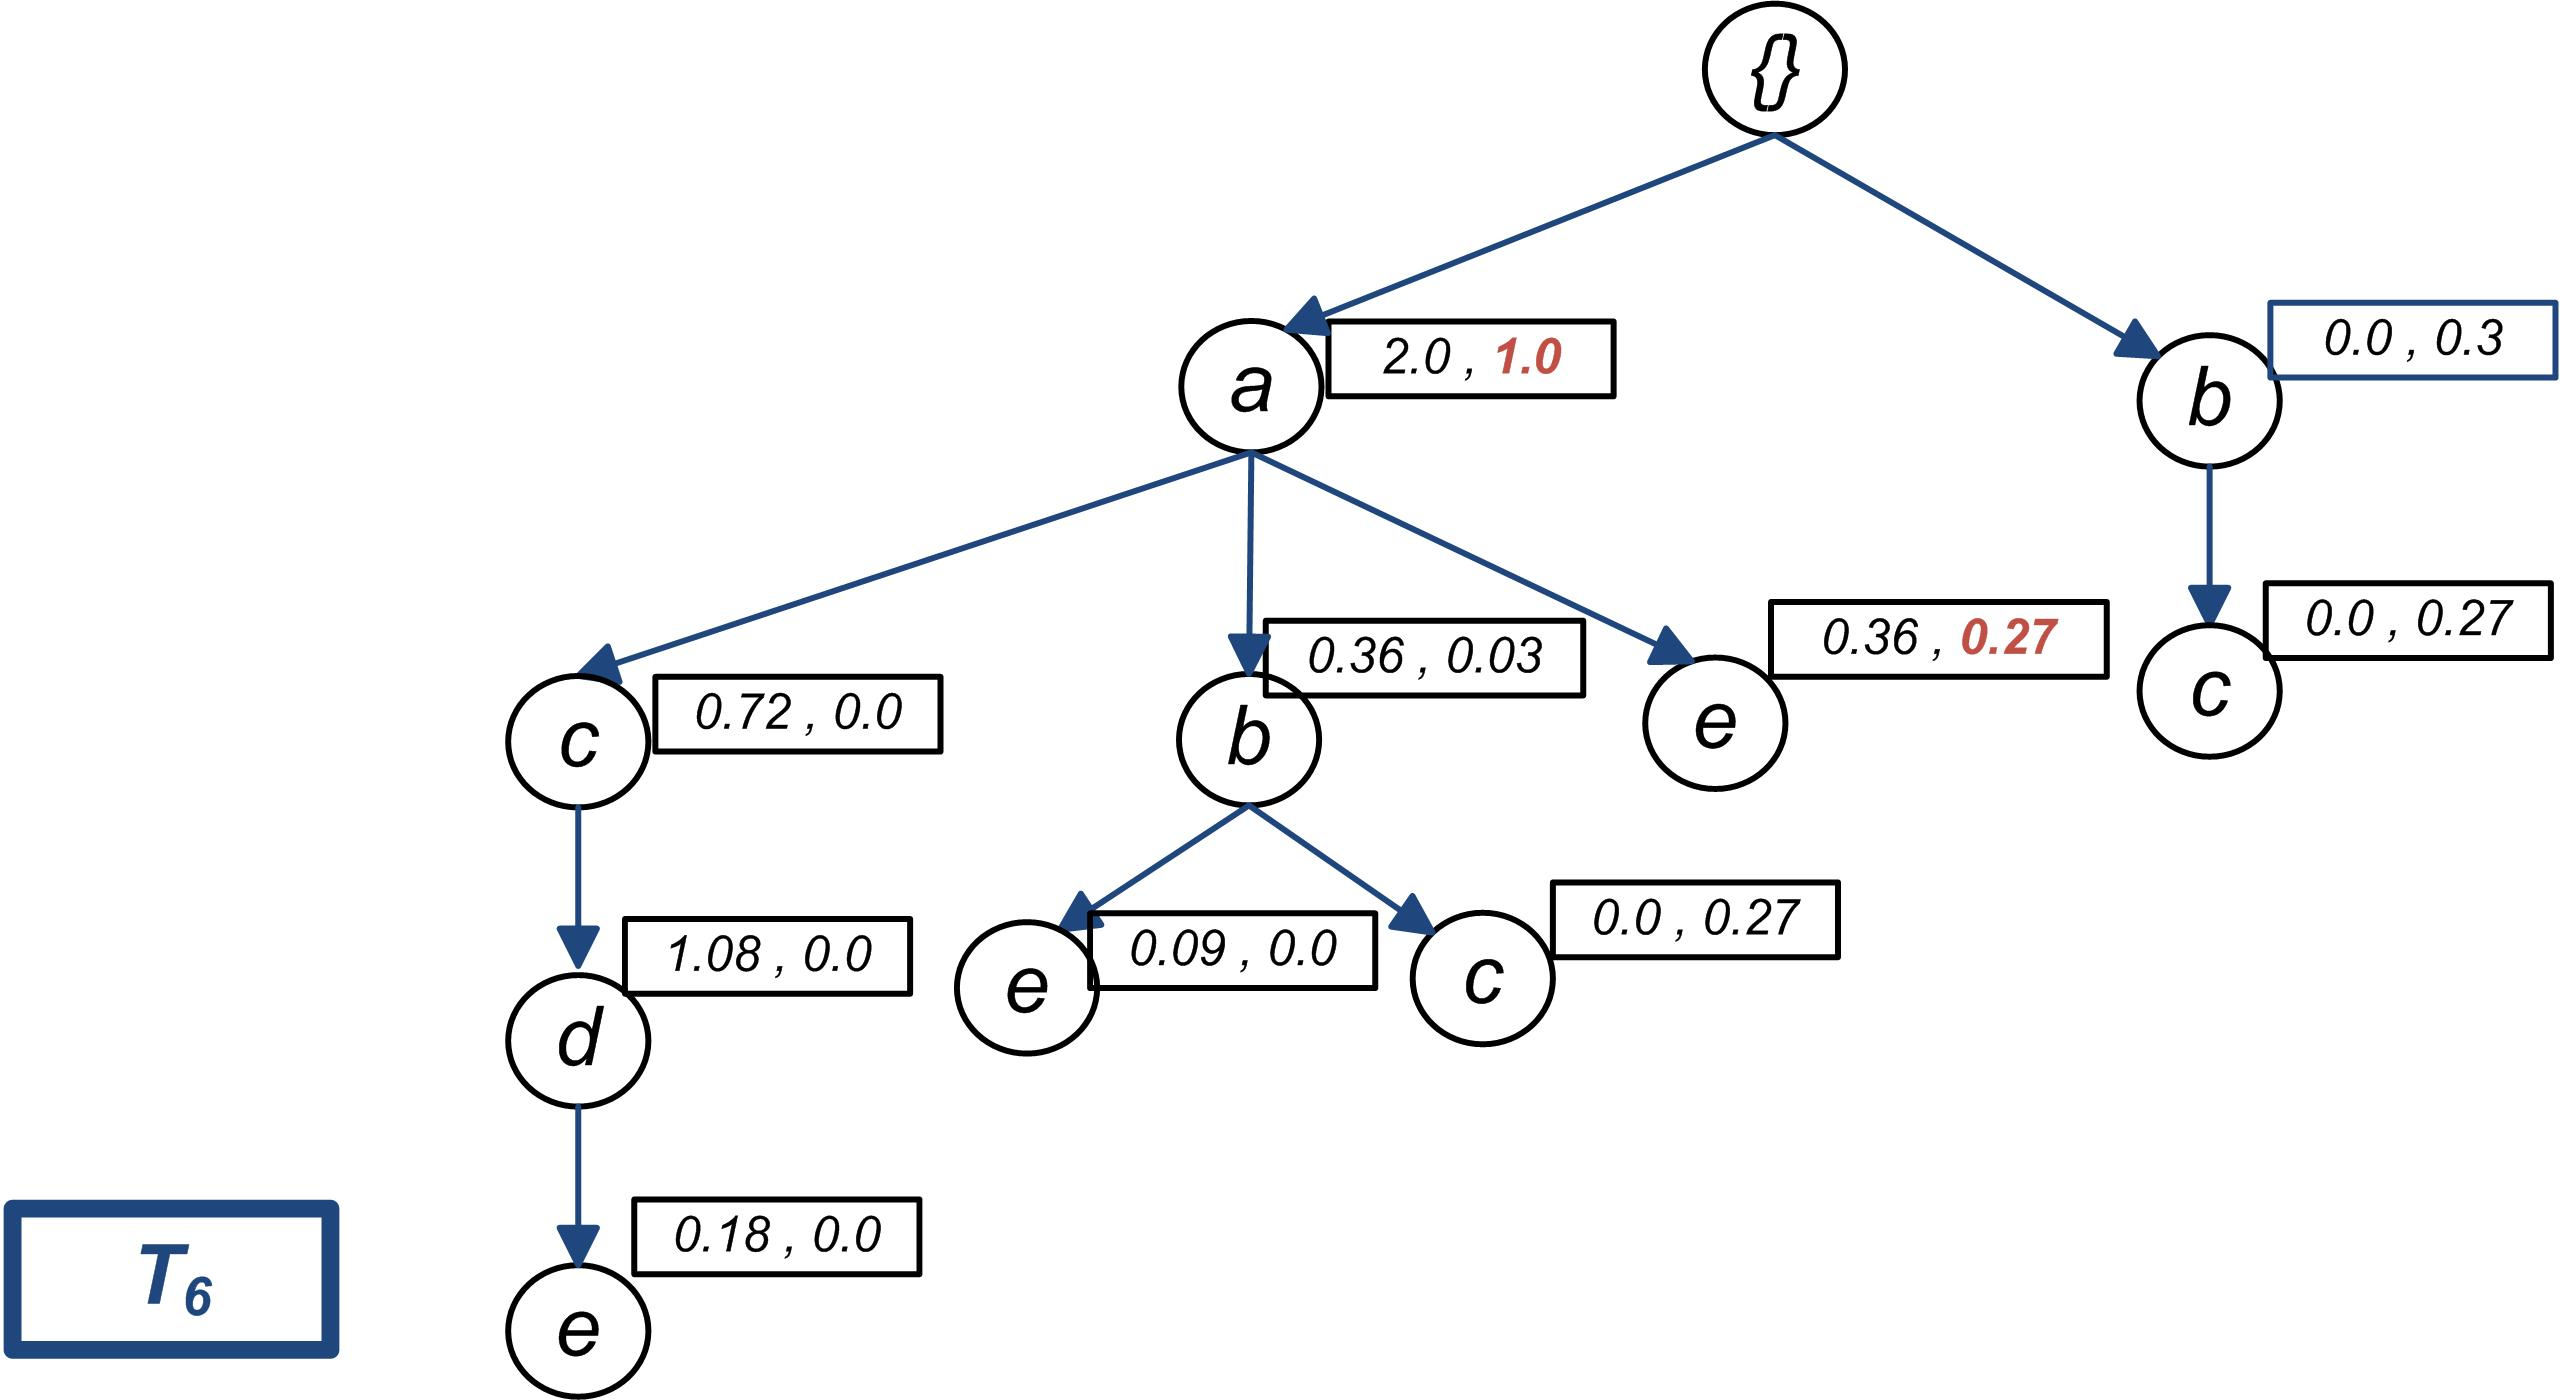
\includegraphics[width=\textwidth,height=3.0cm]{images/sim_06.jpg}
	    \caption{T\textsubscript{6}}
		\end{subfigure}
	}
 \caption{Inserting \emph{T\textsubscript{4}},\emph{T\textsubscript{5}} and \emph{T\textsubscript{6}} in \emph{US-tree}}
 \label{figure:t456}
\end{figure}
\end{frame}
%\end{document}
    Let construct tree for Table-\ref{table:prefix_assigned}. First we insert \emph{Batch-1 (T\textsubscript{1}, T\textsubscript{2}, T\textsubscript{3})} in the window 1. First when inserting the \emph{T\textsubscript{1} - a(0.9), c(0.54), d(0.45), e(0.18)} we insert item \emph{a(0.9)} as a child of root \emph{\{\}} (Figure-\ref{figure:t1}). Update a's prefix value as $0.9$. Then we add \emph{c(0.54)} as a's child update c's prefix value as $0.54$. Aad \emph{d(0.45)} as c's child update d's prefix value as $0.45$. Add \emph{e(0.18)} as d's child update e's prefix value as $0.18$. Thus \emph{T1} is inserted into the tree (Figure-\ref{figure:t1}). For \emph{T\textsubscript{2} - a(0.9), b(0.36), e(0.09)} first we insert \emph{a(0.9)}. Here we found \emph{a} is already inserted so we just update existing node a's prefix value $0.9 + 0.9 = 1.8$ (Figure-\ref{figure:t23}). Then we insert \emph{b(0.36)}. As \emph{a} has no child \emph{b} we insert a new child b and update its prefix value $0.36$. Then insert new e(0.09) as the child of \emph{b}. For \emph{T\textsubscript{3} - a(0.2), c(0.18), d(0.63)} we follow the existing path \emph{a(1.8), c(0.54), d(0.45)} and update corresponding prefix value as $1.8 + 0.2 = 2.0$, $0.54 + 0.18 = 0.72$ and $0.45 + 0.63 = 1.08$ (Figure-\ref{figure:t23}). After inserting the This \emph{T\textsubscript{3}} window 1 is completed. Then we will go for inserting next batch \emph{Batch-2 (T\textsubscript{4}, T\textsubscript{5}, T\textsubscript{6})} in the tree. For \emph{Batch-2} we shall put prefix value in the window's newest place. And thus the latest batch becomes the most recent information. For inserting \emph{T\textsubscript{4} - b(0.3), c(0.27)} we insert new node \emph{b} as there is no child b of root node \emph{\{\}}. So we insert \emph{b} as a child of root \emph{\{\}}. Update its prefix value as $0.3$. Then insert \emph{c(0.27)} as child of \emph{b} and update prefix value $0.27$. Here as this \emph{T\textsubscript{4}} is inserting in \emph{Batch-4} we update prefix value for recent batch's information. Next we insert \emph{T\textsubscript{5} - a(0.1), b(0.03), c(0.27)}. We merge \emph{a(0.1), b(0.03)} with previous \emph{a, b } nodes and update prefix value $0.1$ and $0.03$ in the second batch's portion and insert new node \emph{b} as a child of \emph{b} and update its prefix value as $0.27$ (Figure-\ref{figure:t456}).
    %\documentclass{article}
%\usepackage{graphicx}
%\usepackage{caption}
%\usepackage{subcaption}
%
%\begin{document}
\begin{figure}
  \centering
	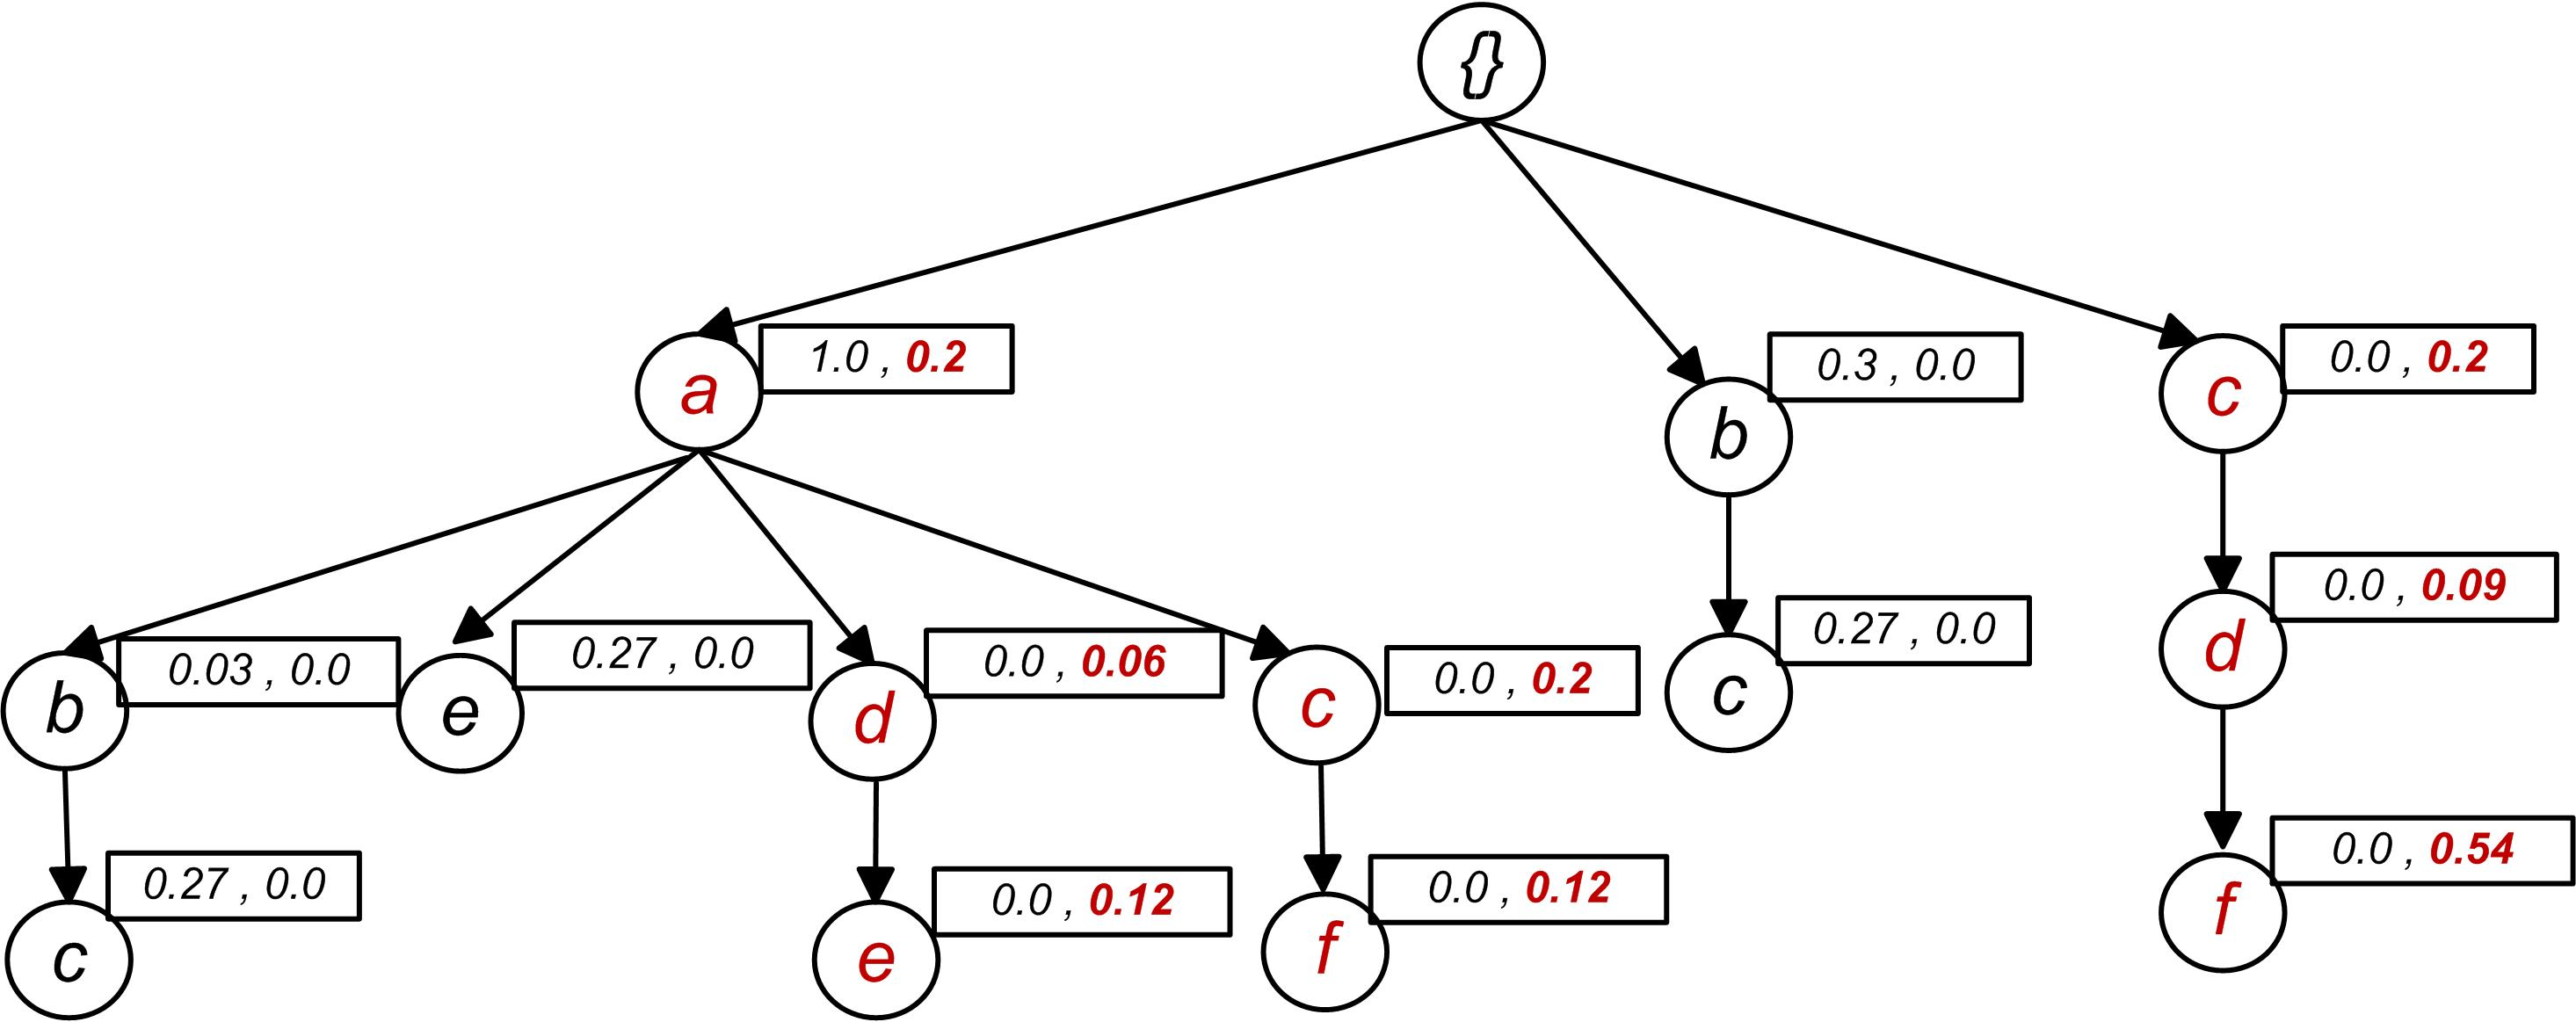
\includegraphics[width=.8\textwidth]{images/sim_789.jpg}  
	\caption{Inserting \emph{T\textsubscript{7}, T\textsubscript{8}, T\textsubscript{9}} into \emph{US-tree} after sliding}
	\label{figure:w2}
\end{figure}
%\end{document}
    Now our window is completed and can our \emph{USFP-growth} mine \emph {US-tree}. When new transaction batch comes like \emph{Batch-3 (T\textsubscript{7}, T\textsubscript{8}, T\textsubscript{9})} comes to be inserted into the tree then first we have to slide the window. For this when we construct the tree we maintain a header table which contains the information for the oldest data. Thus pointer points to the oldest data can be found easily and slide the whole tree. Figure-\ref{figure:slide} shows the sliding and getting the old data removed tree and ready to insert next batch \emph{Batch-3}. After inserting \emph{Batch-3} we get the tree like Figure-\ref{figure:w2}. 
    \documentclass{article}
\usepackage{graphicx}
\usepackage{caption}
\usepackage{subcaption}

\begin{document}

\begin{frame}

\begin{figure}[!tbp]
  \centering
	\fbox{  
	 	\begin{subfigure}[b]{0.44\textwidth}
	 	\centering
	    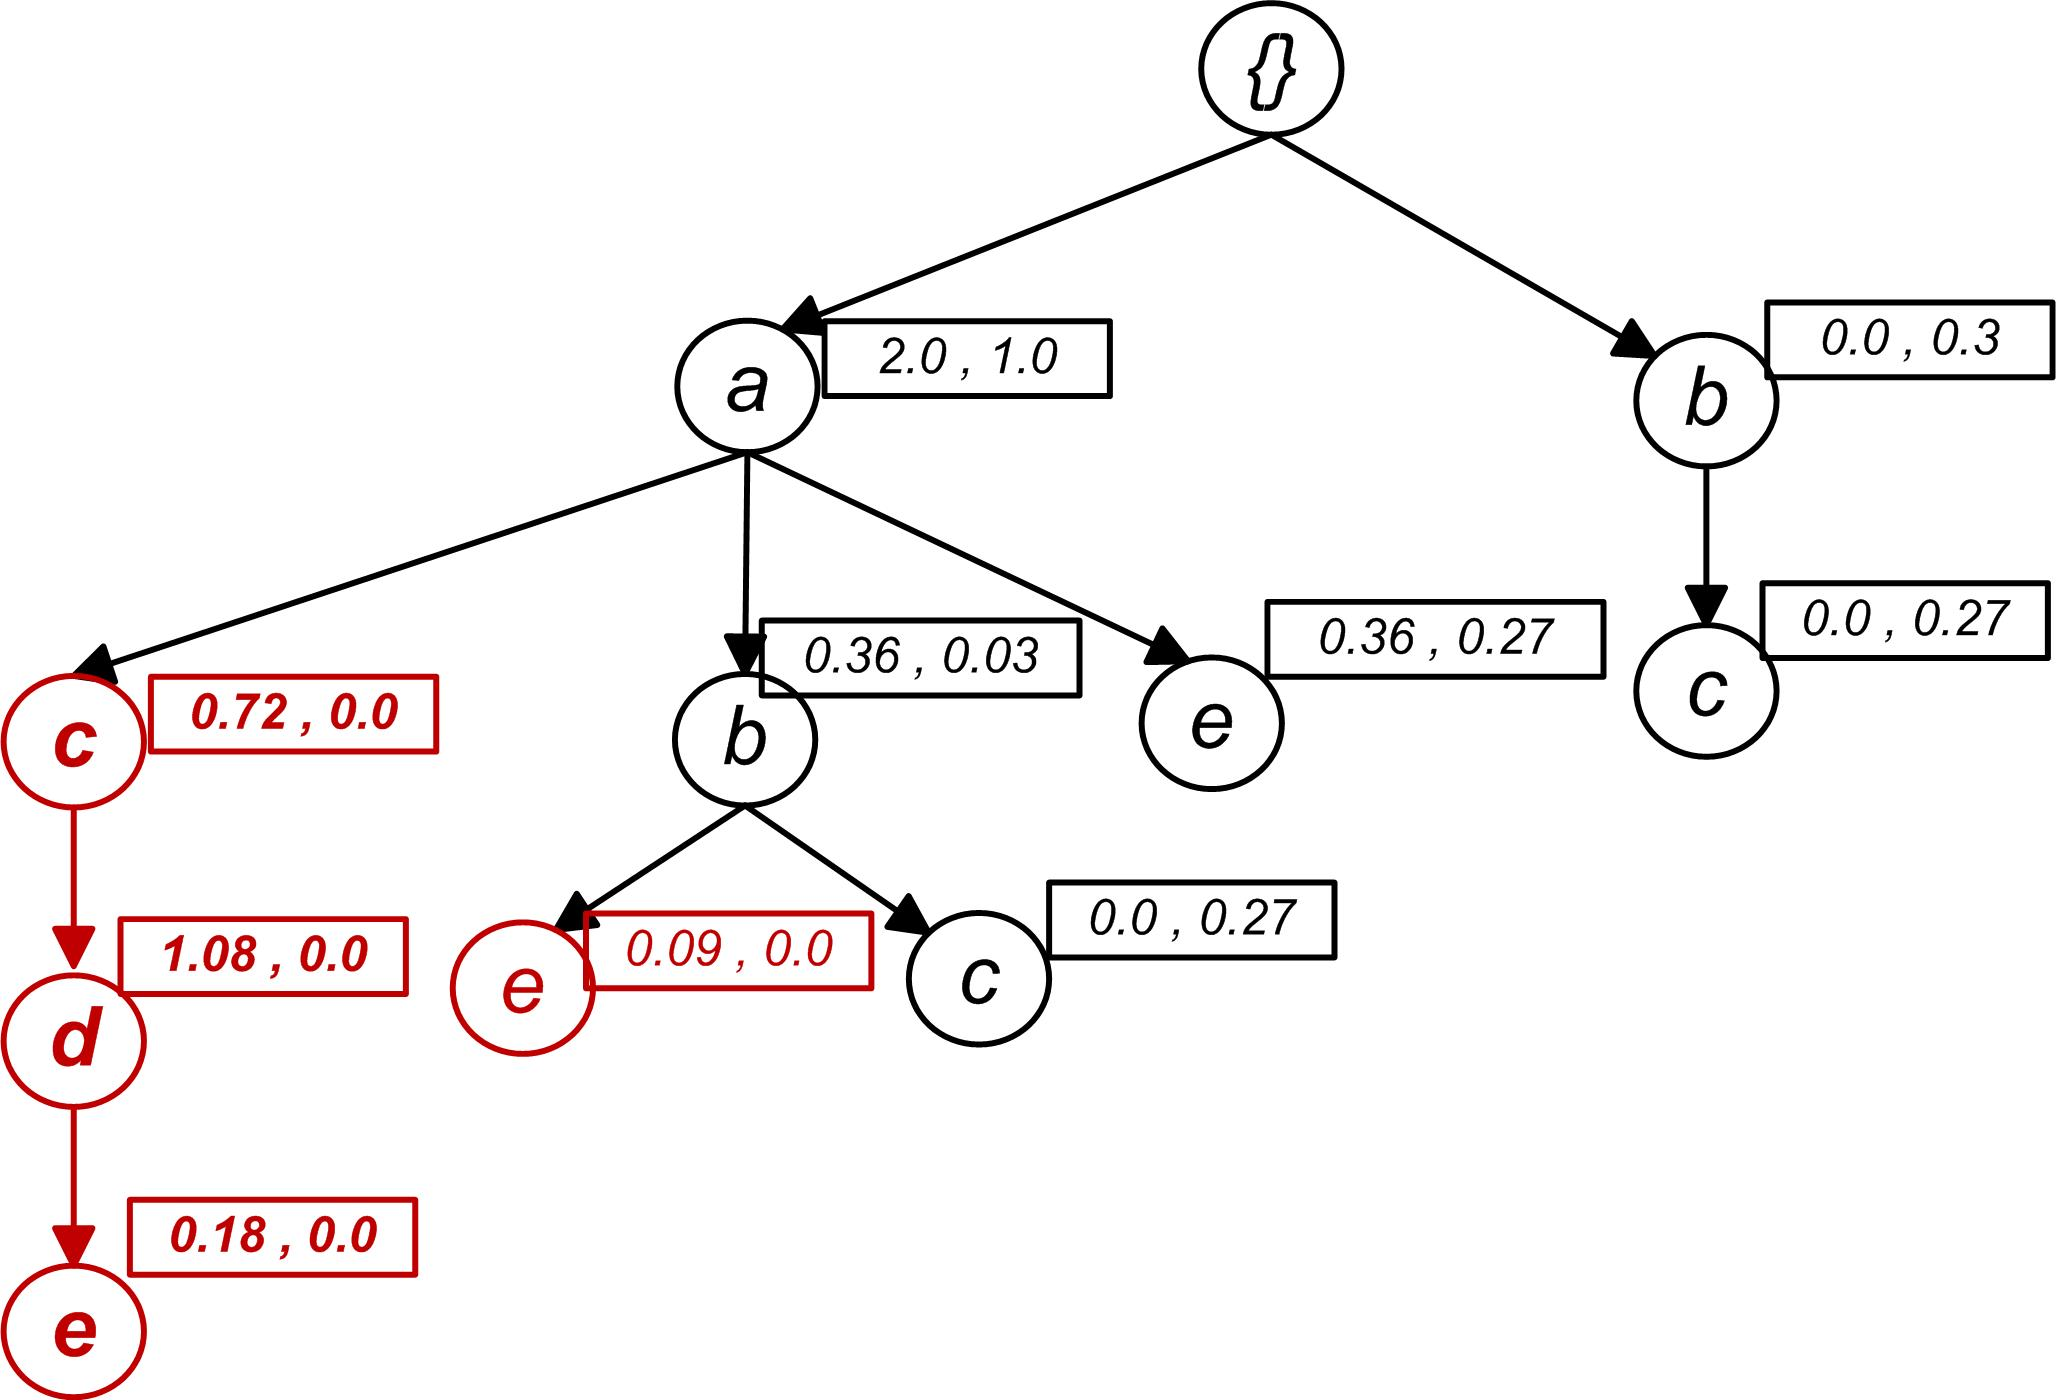
\includegraphics[width=\textwidth,height=4.5cm]{../images/sim_06_slide.jpg}
	    \caption{Before Sliding}
		\end{subfigure}
 
	 	\begin{subfigure}[b]{0.36\textwidth}
	 	\centering
	    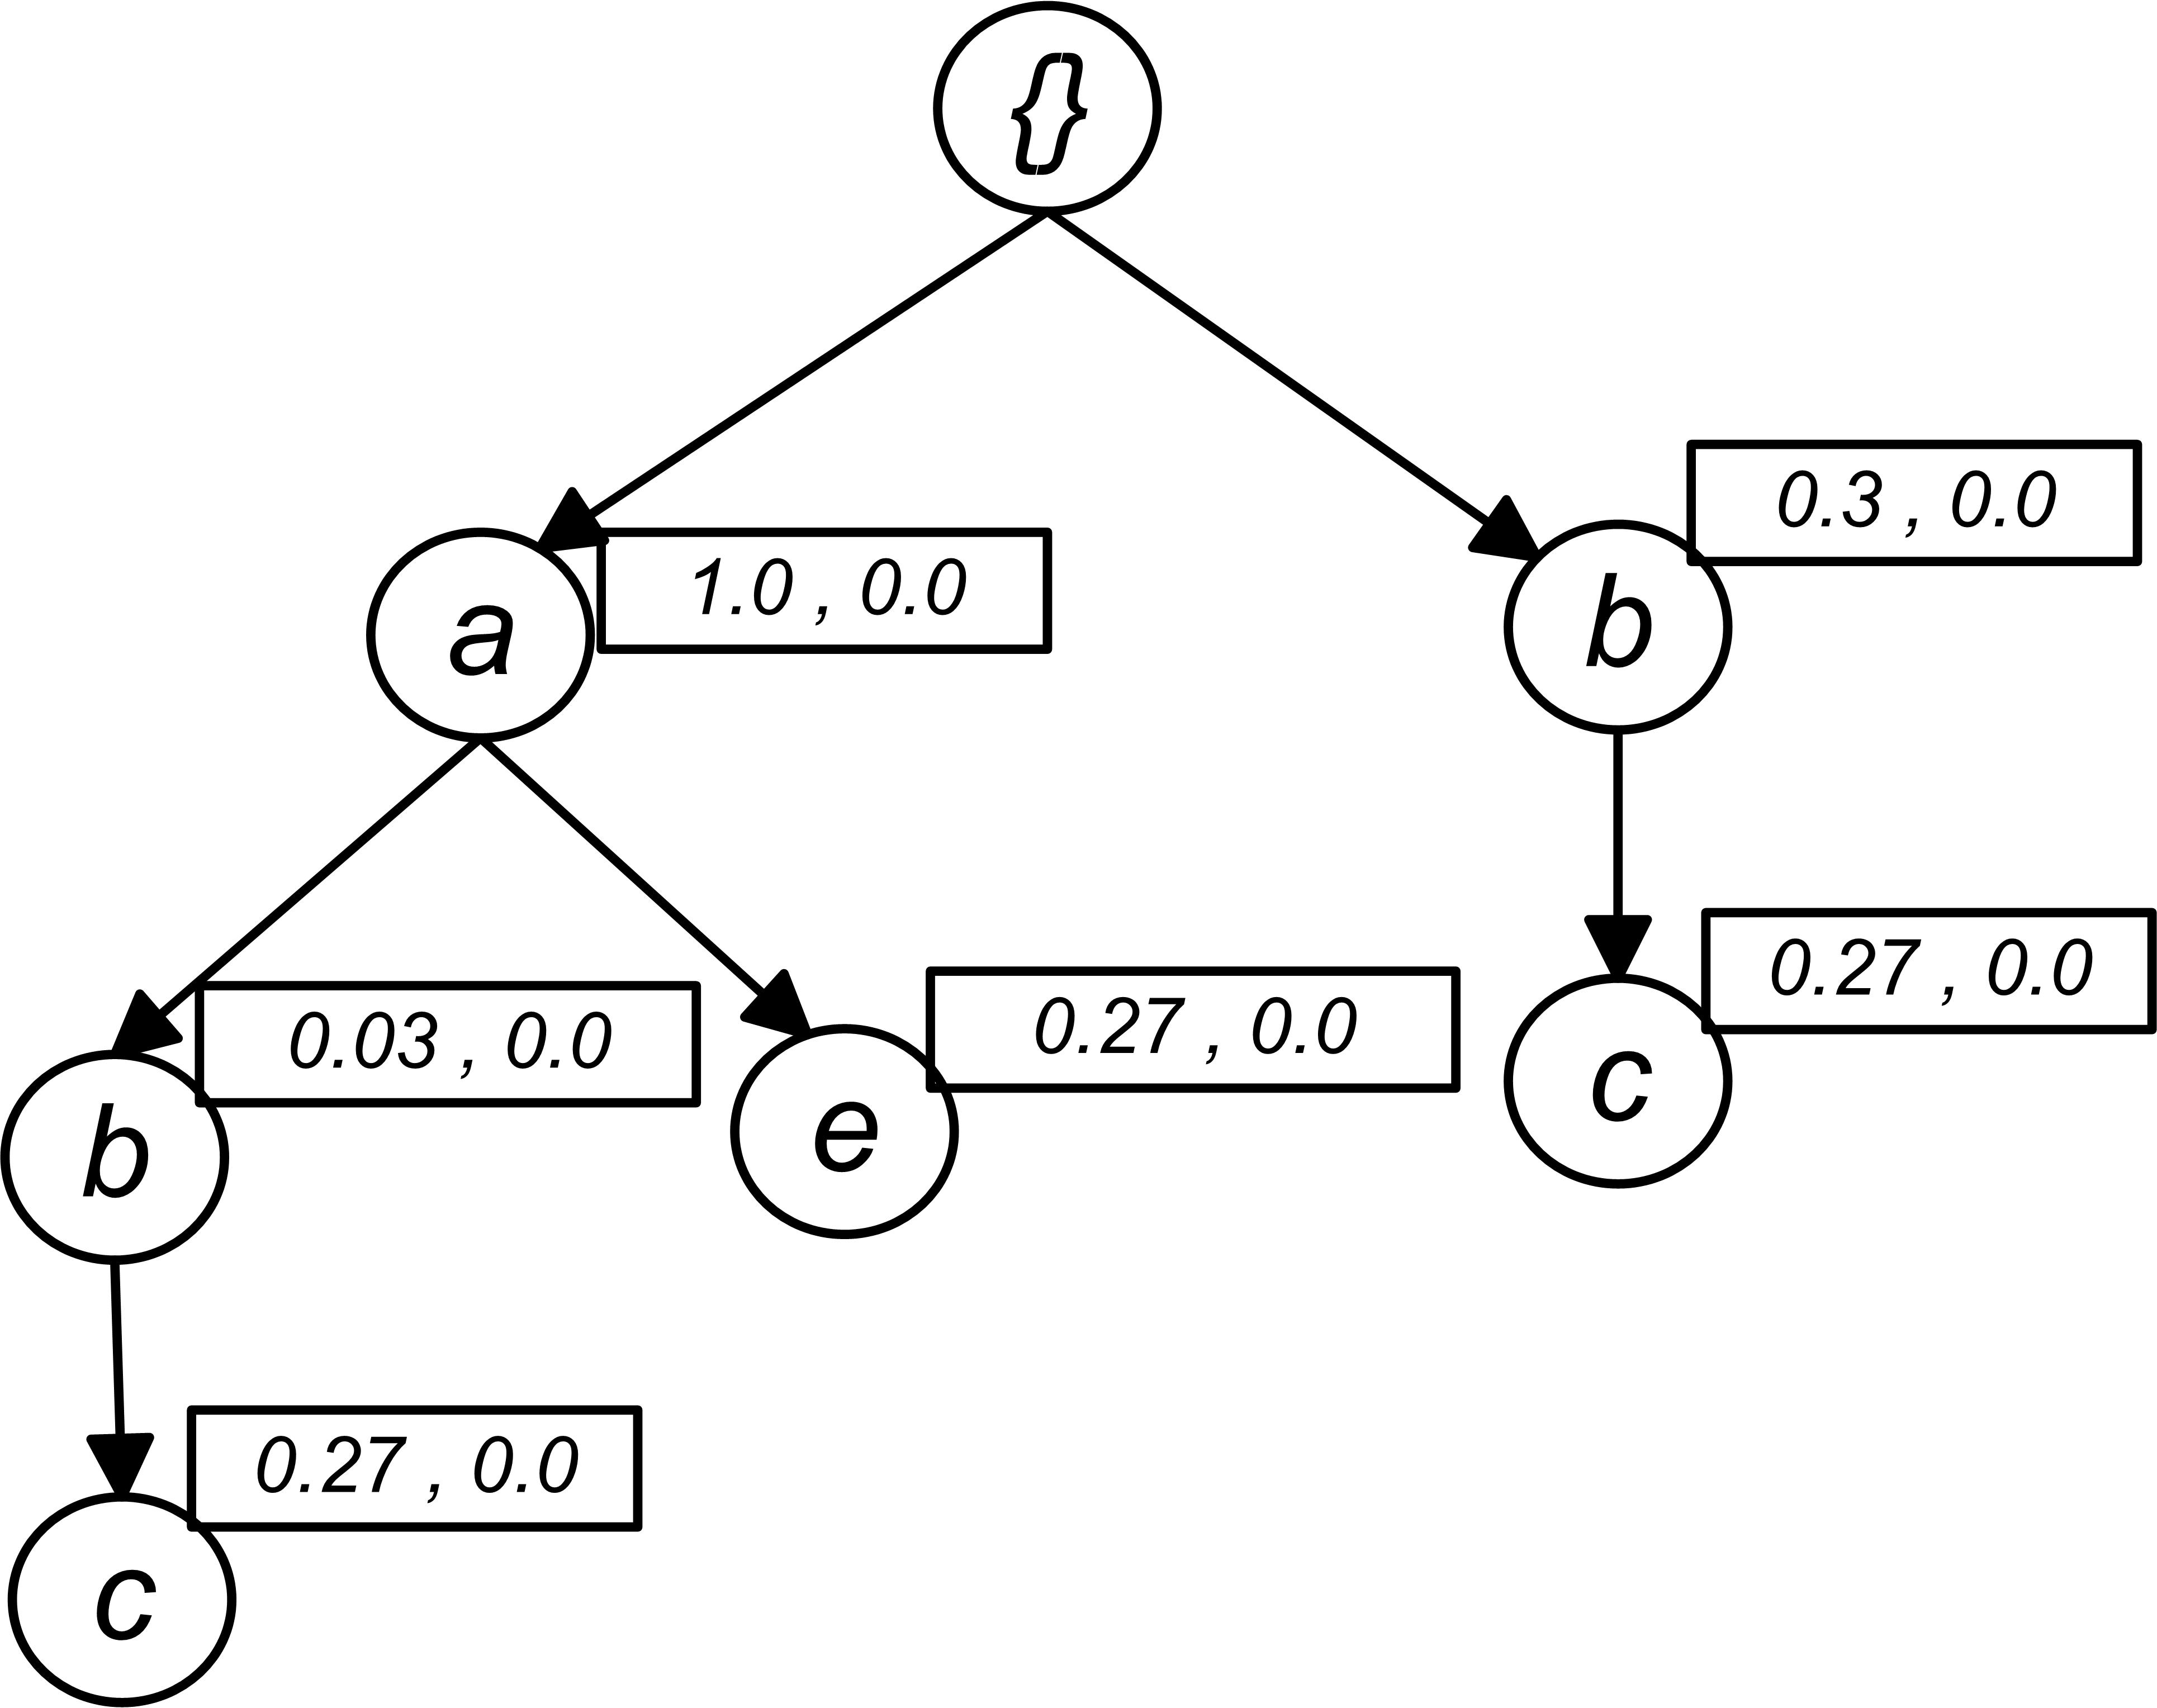
\includegraphics[width=\textwidth,height=4.5cm]{../images/sim_06_slide_2.jpg}
	    \caption{After Sliding}
		\end{subfigure}
	}
 \caption{Sliding \emph{US-tree}}
\end{figure}
\end{frame}



\end{document}
    In the described \emph{US-tree} construction process we see that tree sharing is very much common and regular. That makes our tree very compact and memory needed to hold items becomes less. Moreover, the tree construction time improves surprisingly. When to mine this \emph{US-tree} we can gain a lot time when mining. As the tree size is small, conditional tree will be much more less when mining. We will gain a lot time when trying to mine the conditional trees. In the experimental result section we will provide necessary graphs for our simulations.
    \subsection{Mining US-tree FPUS-growth}
    In this section we will discuss about our mining algorithm \emph{USFP-growth} (algorithm-\ref{algorithm:mine}) That will find frequent patterns. For mining we used \emph{FP-growth} like approach. Generally, we can remove all the nodes having support less than \emph{minimum support}. From header table we get such information that which nodes is less than \emph{minimum support}. We told earlier that for \emph{U\textsuperscript{cap}} value we took the upper limit, we also can we can remove all the nodes having prefix value less than \emph{minimum support}. In this process we can eliminate most of the infrequent nodes from tree. For this purpose we used header table that was created when creating the \emph{US-tree}. Then we construct conditional tree starting from the lowest support holding node. From header table we also get the position of all nodes containing same item in the tree. 
    Let’s mine the tree we constructed earlier. Figure-\ref{figure:min_before} is \emph{US-Tree} for mining and corresponding header table before starting mining. From the header table, we get that support of \emph{a} is $3.00$, \emph{b} is $1.00$, \emph{c} is $3.30$, \emph{d} is $1.20$, \emph{e} is $0.60$. So, \emph{e} is not frequent for one item set frequent pattern. So it is sure that no item set contains \emph{e} will be frequent. That is the basic upward closure property of frequent item set. So we remove all the nodes of \emph{e} and get the new mining tree Figure-\ref{figure:min_ready} and its header table. Here we find all one item sets that are frequent and that is \emph{\{a\}, \{b\}, \{c\} \{d\}} Now we will construct conditional tree for the found frequent one item and mine the conditional tree. But items having total \emph{U\textsuperscript{cap}} less than \emph{minimum support} is not needed to construct conditional tree because this \emph{U\textsuperscript{cap}} value has been take as the upper bound. So total \emph{U\textsuperscript{cap}} value less than \emph{minimum support} indicates that item must not be exists in the $2$ or more frequent item set. So we do not construct conditional tree for these items.
    We construct conditional tree from items having lowest total \emph{U\textsuperscript{cap}} value greater than \emph{minimum support}. As \emph{b} having total \emph{U\textsuperscript{cap}} is $.69$ \emph{b}, is ignored for constructing conditional tree. Then the next candidate is \emph{d}. From header table pointer we find that there is only one path item \emph{d} exists in the mining tree Figure-\ref{figure:min_ready}. That is \{\emph{a, c, d}\}:$1.08$. So we create conditional tree and update all nodes mining probability with \emph{d's} \emph{U\textsuperscript{cap}} $1.08$. For this conditional tree Figure-\ref{figure:d_cond} the header tables says all the nodes in the tree are having \emph{U\textsuperscript{cap}} greater than \emph{minimum support} $.9$. So, all the items are ready to be constructed as conditional tree. As here is only one branch so we do not further construct conditional tree and take all the combinations as frequent items Figure-\ref{figure:d_cond} Table. So we find \emph{\{dc\}, \{da\}, \{dca\}} as frequent pattern. Next we create conditional tree for \emph{c}. Here c exists in the tree for three path those are \emph{\{a, c\} : $0.72$ , \{a , b, c\} : $.027$ and \{b, c\} : $0.27$}. So we create conditional tree (Figure-\ref{figure:c_cond}). Total mining value of \emph{c} is the sum of item caps in each respective path of \emph{c}. From the header we see that \emph{b} has total cap having less than \emph{minimum support} so we remove \emph{b} and create two item set \emph{\{ca\}}. Next we construct \emph{ca} conditional tree that contains only root (\emph{\{\}}). So no further tree is needed to be constructed and minned. Than we create conditional tree for \emph{a}. And find only root \emph{\{\}}. Thus we get all the frequent patterns. All the patterns are \emph{\{a\}, \{b\}, \{c\} \{d\}, \{dc\}, \{da\}, \{dca\} and \{ca\}}. As we have found all patterns from upper bound, so that it is guaranteed that there will be no false negative. But some false positive can be exists in the found frequent item set as there may be some value less than max value we assumed. So in the next section we will show an approach that eliminates the all false positives (if exists) in the data set.
    %\documentclass{article}
%\usepackage{caption}
%\usepackage{graphicx}
%\begin{document}

\begin{figure}
\begin{minipage}{0.40\textwidth}
  \centering
  
	\begin{center}
	\begin{tabular}{ |c|c|c| } 
 	\hline
 		Item&\emph{U\textsuperscript{cap}}&Support\\ \hline\hline
 		a &  3.00  & 3.00	\\ \hline
 		c &  1.26  & 3.30	\\ \hline
 		d &  1.08  & 1.20	\\ \hline
 		e &  0.54  & 0.60	\\ \hline
 		b &  0.69  & 1.00	\\ \hline
\end{tabular}
\end{center}   
  \captionof{table}{Header Table of US-tree}
\end{minipage}
\hfill
\begin{minipage}{0.40\textwidth}
  \centering
  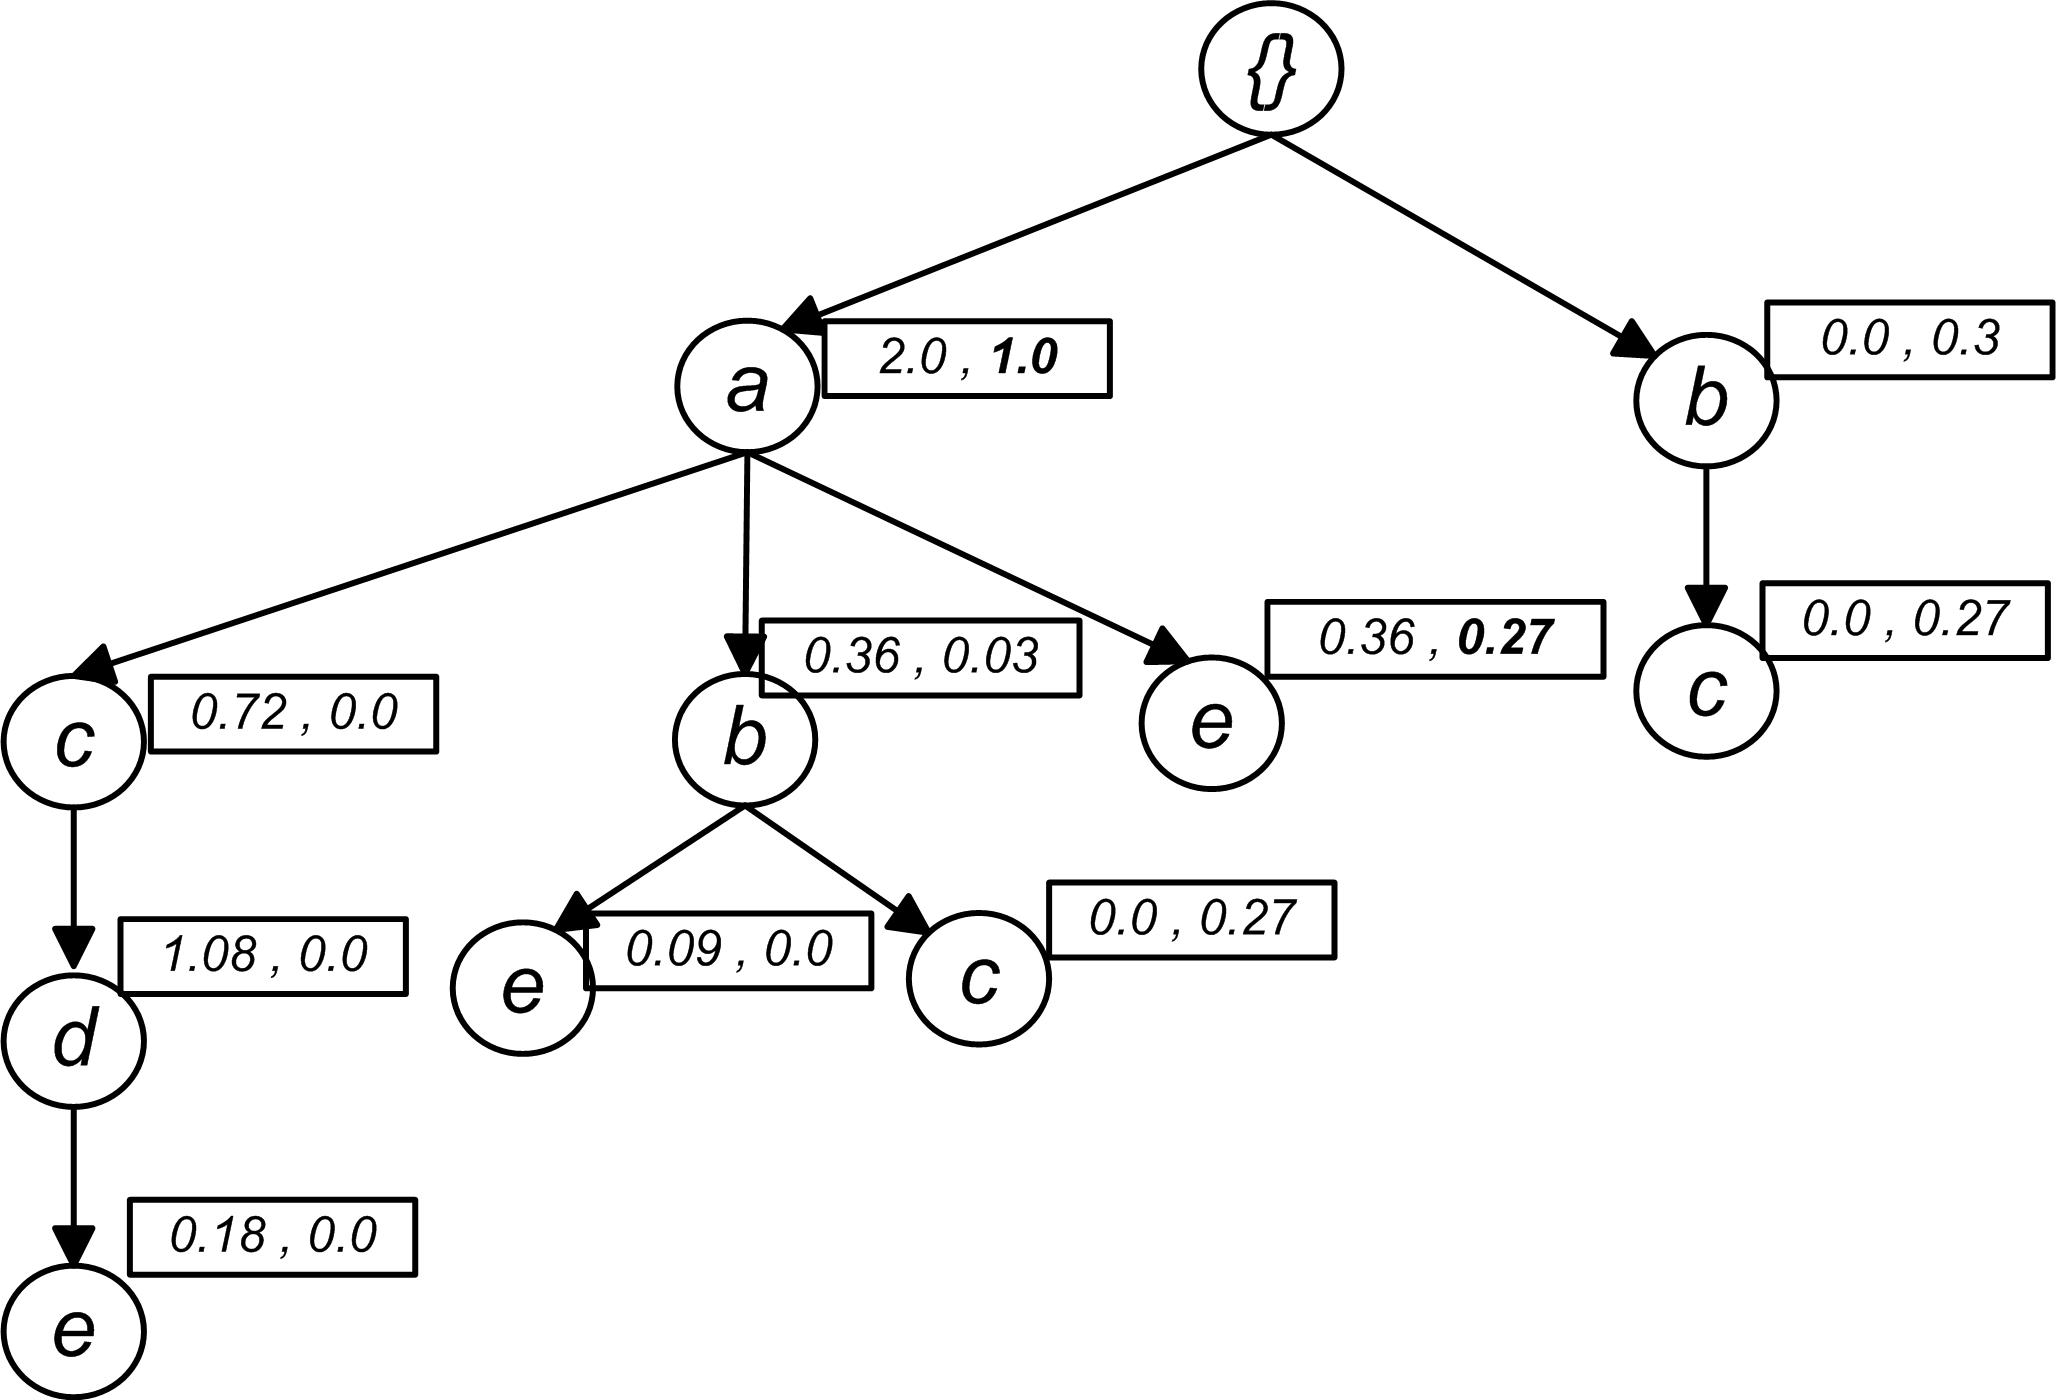
\includegraphics[width=\textwidth]{images/us_tree.jpg}
  \captionof{figure}{US-tree}
\end{minipage}
\caption{US-tree and Header Table}
\label{figure:min_before}
\end{figure}


\begin{figure}
\begin{minipage}{0.40\textwidth}
  \centering
  
	\begin{center}
	\begin{tabular}{ |c|c|c| } 
 	\hline
 		Item&\emph{U\textsuperscript{cap}}&Support\\ \hline\hline
 		a &  3.00  & 3.00\\ \hline
 		c &  1.26  & 3.30\\ \hline
 		d &  1.08  & 1.20\\ \hline
 		b &  0.69  & 1.00\\ \hline
\end{tabular}
\end{center}  
  
  
  \captionof{table}{Header Table for Mining}
\end{minipage}
\hfill
\begin{minipage}{0.40\textwidth}
  \centering
  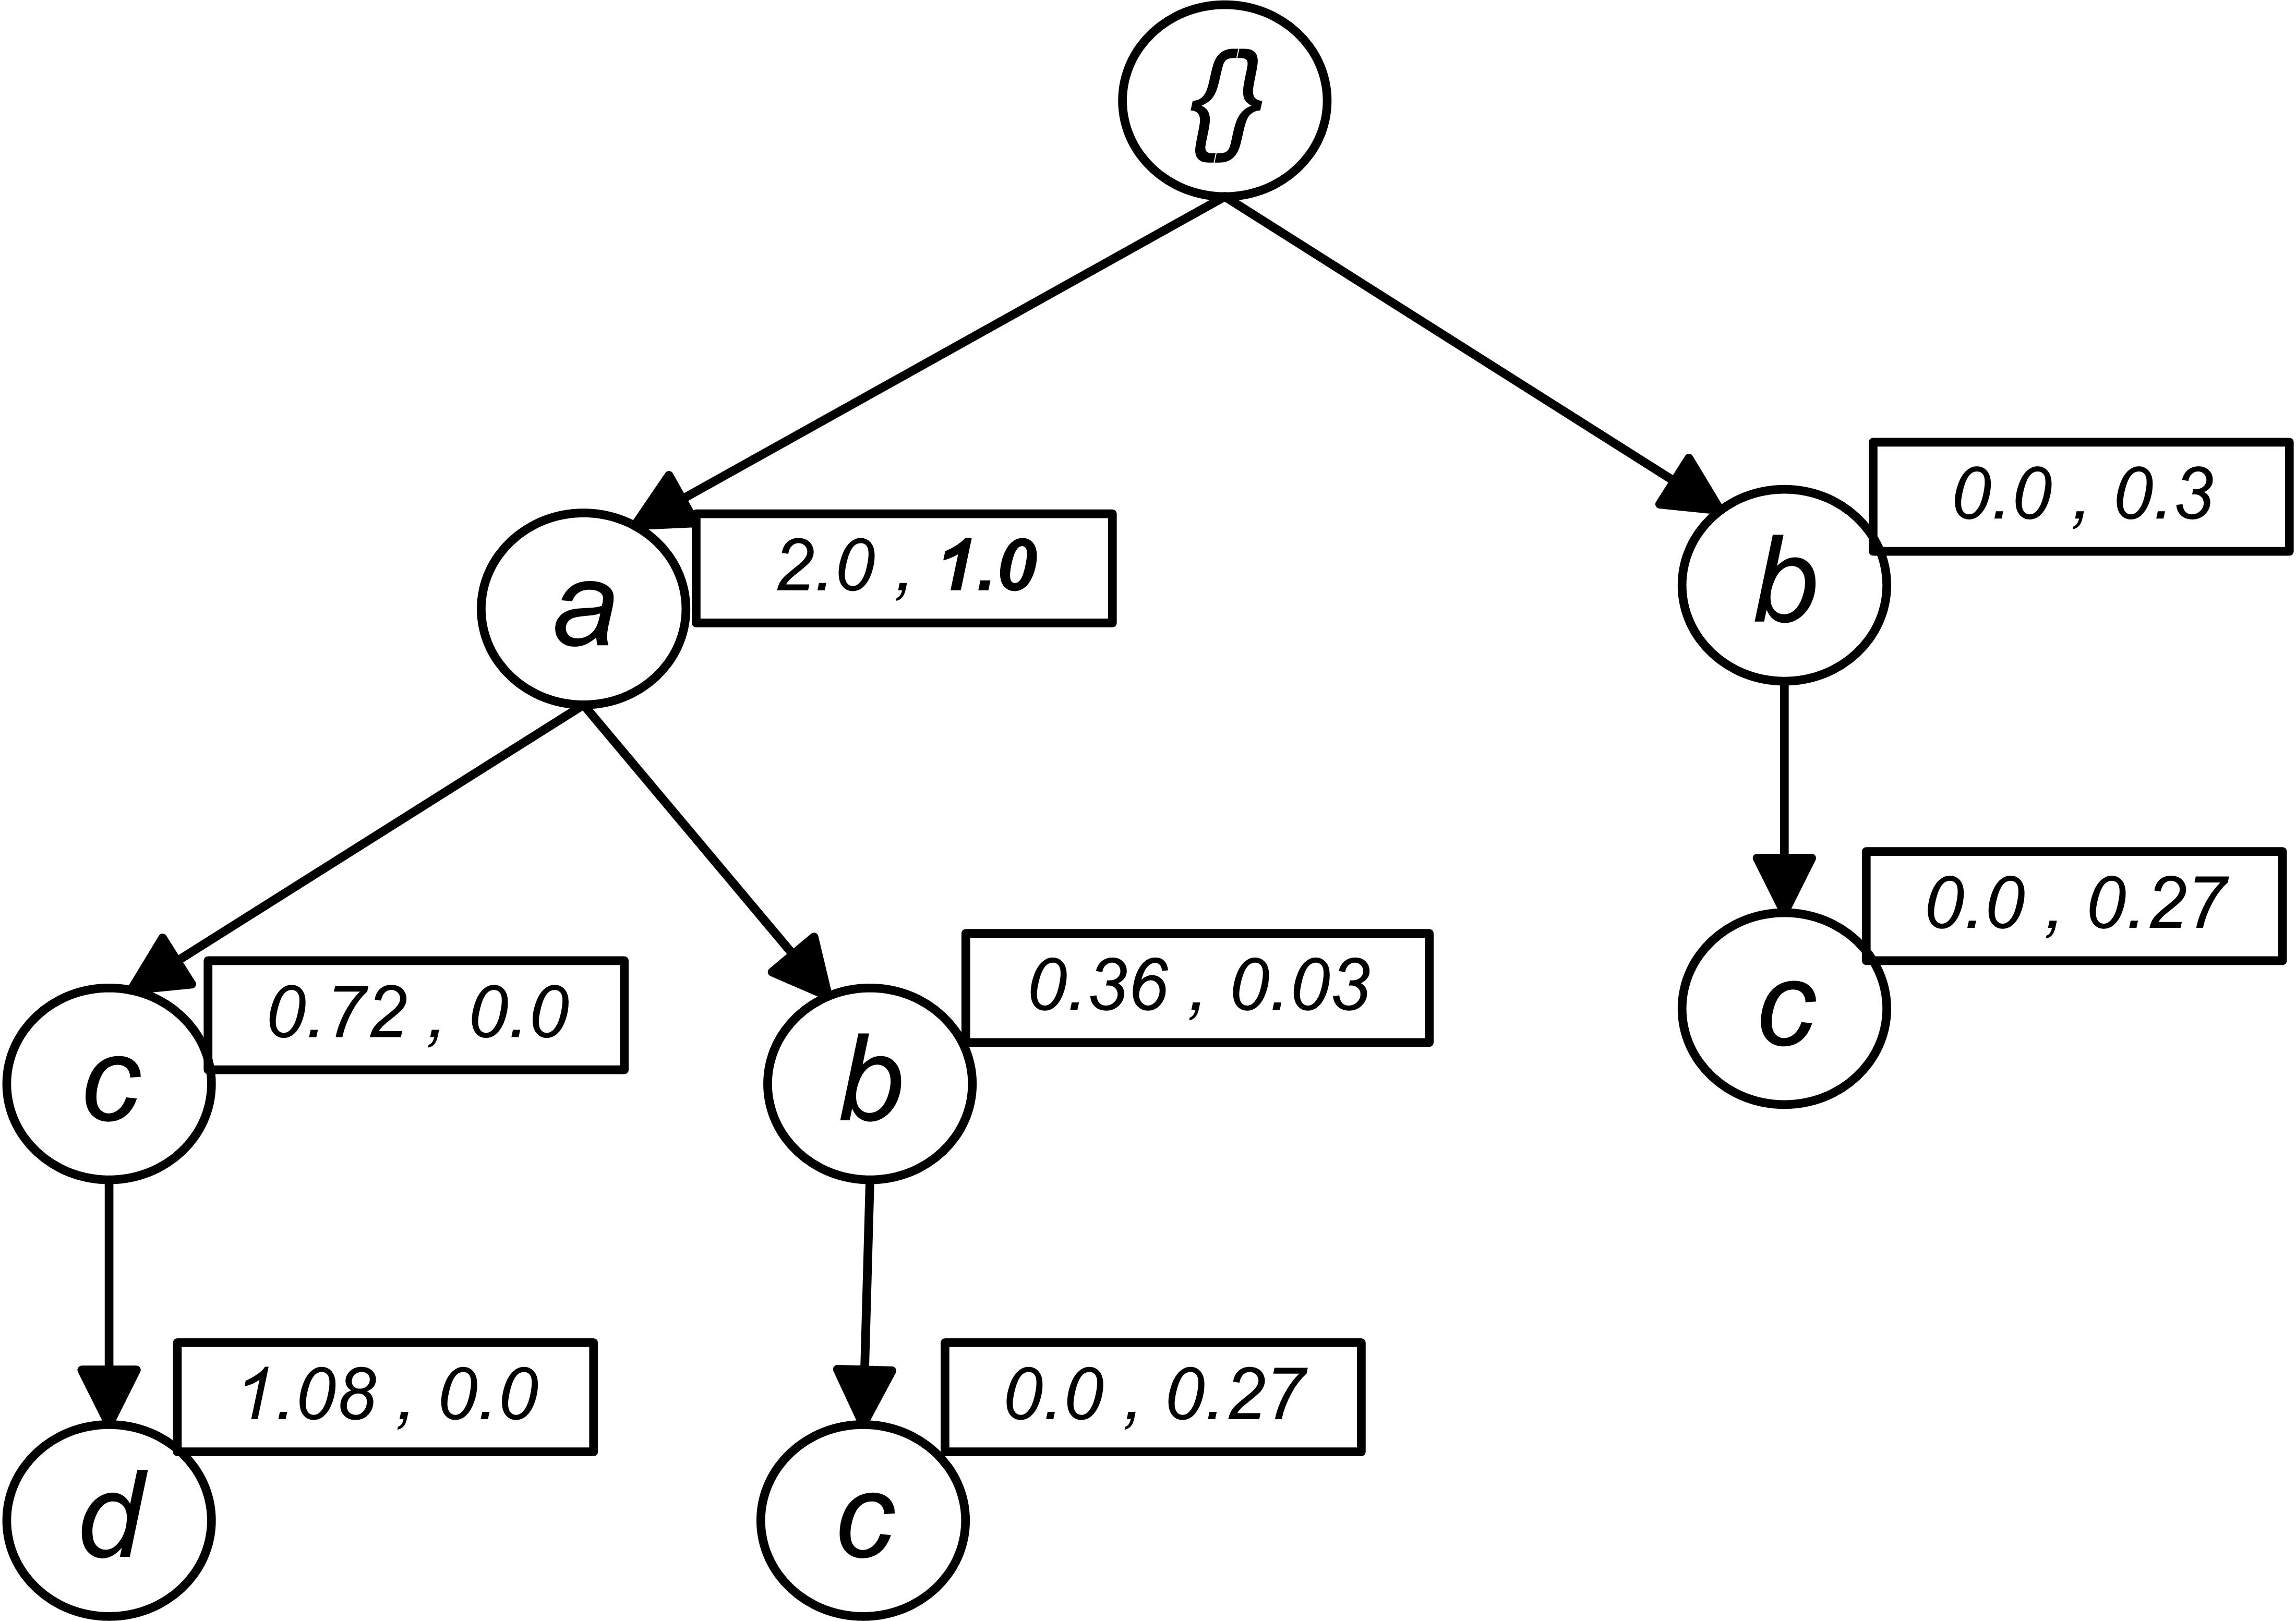
\includegraphics[width=\textwidth]{images/M_TREE.jpg}
  \captionof{figure}{US-tree for Mining}
\end{minipage}
\caption{US-tree and Header Table for Mining}
\label{figure:min_ready}
\end{figure}
%\end{document}
    %\documentclass{article}
%\usepackage{caption}
%\usepackage{graphicx}
%\begin{document}
\begin{figure}
\begin{minipage}{0.40\textwidth}
  \centering
	\begin{center}
	\begin{tabular}{ |c|c| } 
 	\hline
 		Item&Value\\ \hline\hline
 		a &  1.08  	\\ \hline
 		c &  1.08   	\\ \hline
 		
\end{tabular}
\end{center}  
  \captionof{table}{\emph{d-cond tree} Header }
\end{minipage}
  \hfill
\hfill
\begin{minipage}{0.23\textwidth}
  \centering
  \hfill
  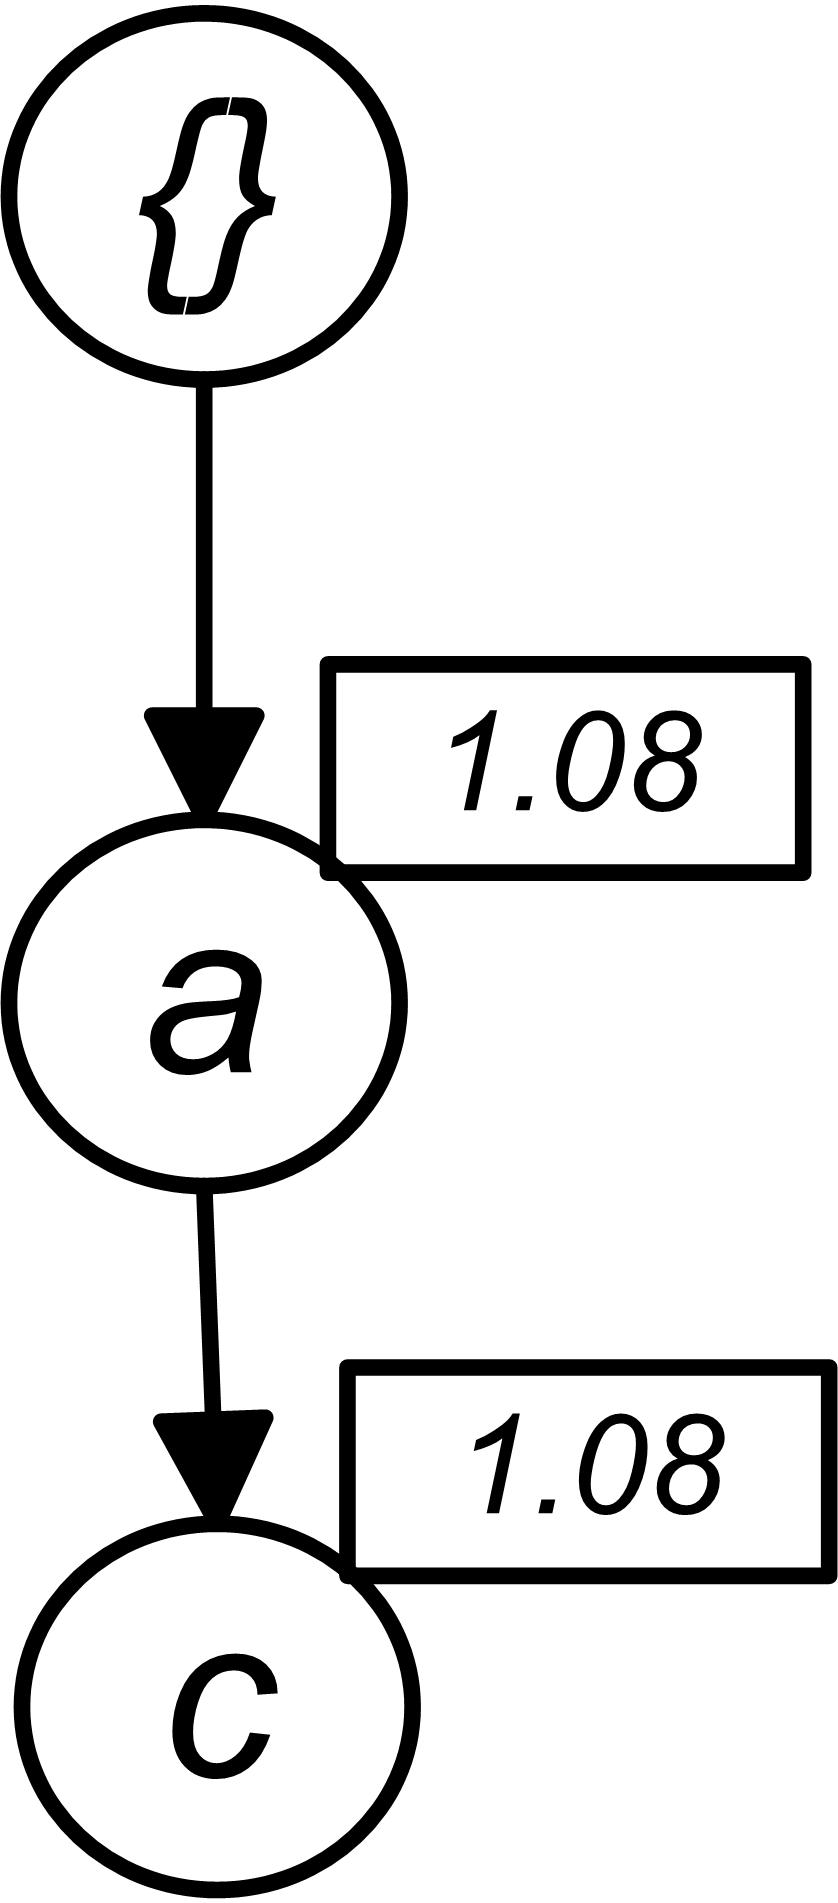
\includegraphics[width=.8\textwidth, height=5cm]{images/D_COND.jpg}
  \hfill
\end{minipage}
\hfill
\begin{minipage}{0.30\textwidth}
  \centering
  
	\begin{center}
	\begin{tabular}{ |c| } 
 	\hline
 		Freq Patterns \\ \hline\hline
 		dc  	\\ \hline
 		da   	\\ \hline
 		dca   	\\ \hline
 		
\end{tabular}
\end{center}  
  \captionof{table}{ \emph{Frequent Patterns} }
\end{minipage}
\caption{\emph{d-cond} Tree and corresponding Header}
\label{figure:d_cond}
\end{figure}
\begin{figure}
\begin{minipage}{0.30\textwidth}
  \centering
	\begin{center}
	\begin{tabular}{ |c|c| } 
 	\hline
 		Item&Value\\ \hline\hline
 		a &  .99  	\\ \hline
 		b &  .54   	\\ \hline
\end{tabular}
\end{center}  
  \captionof{table}{Header }
\end{minipage}
  \hfill
\begin{minipage}{0.29\textwidth}
  \centering
  \hfill
  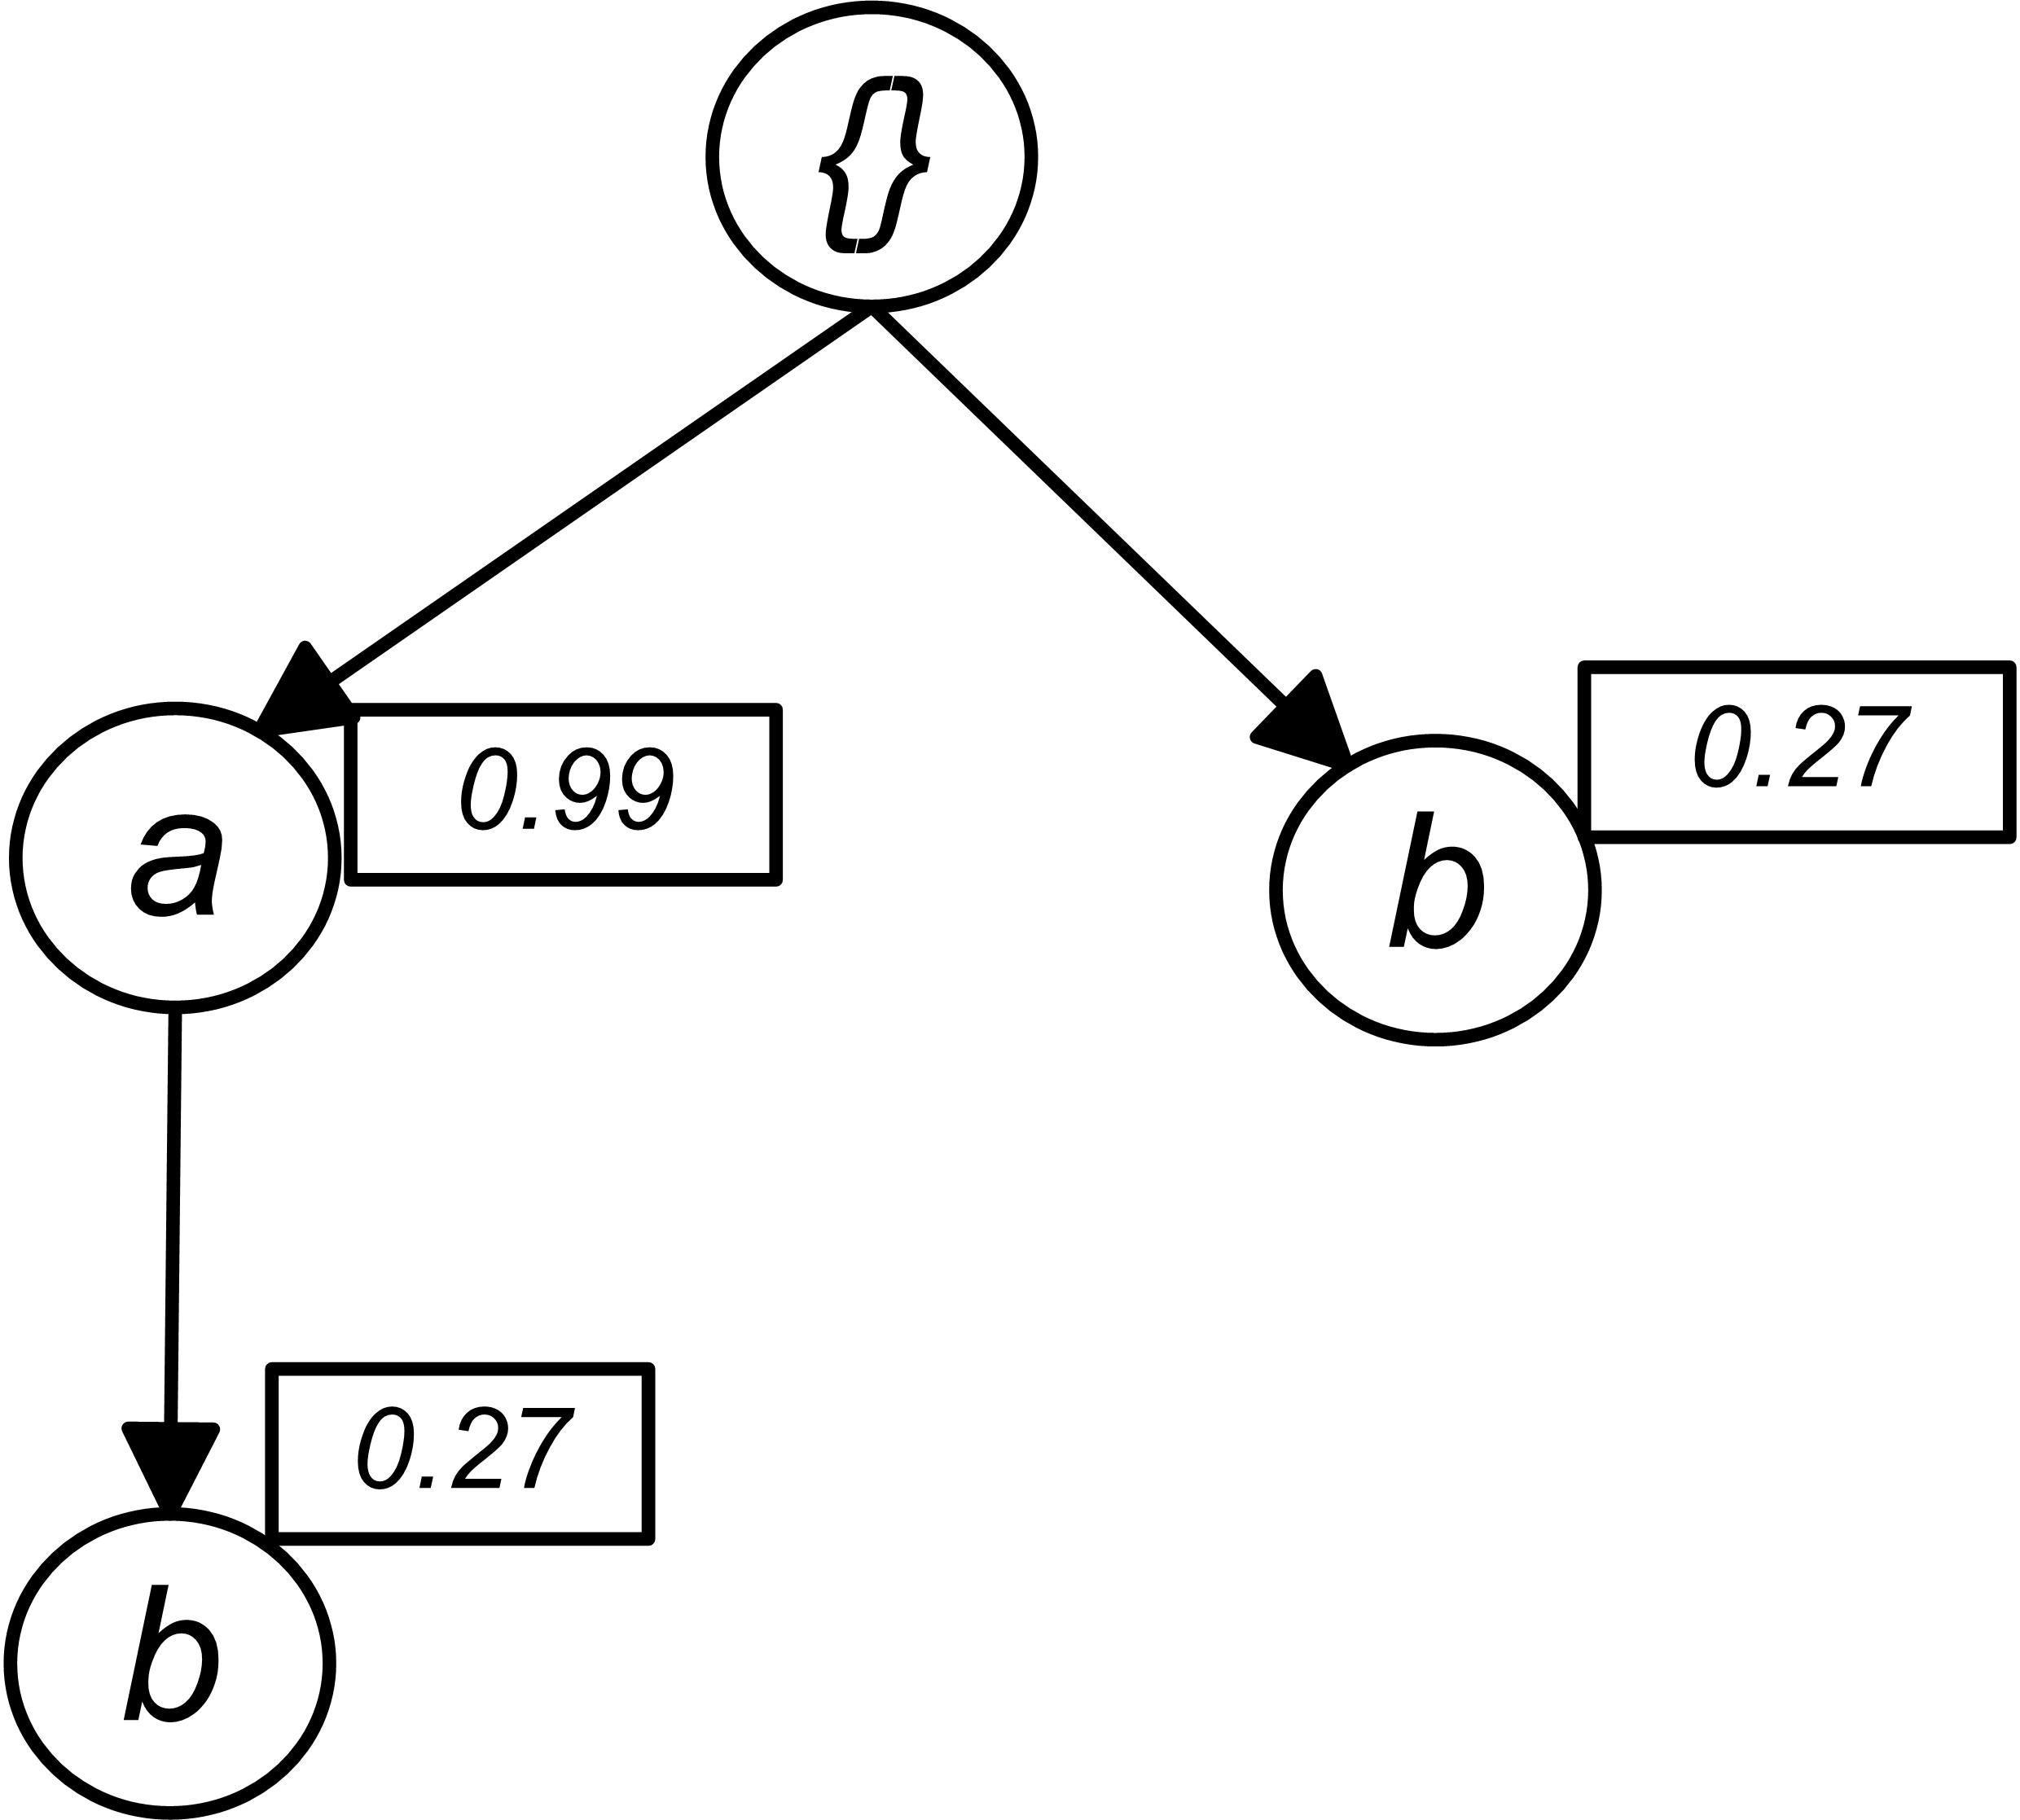
\includegraphics[width=.8\textwidth, height=3.5cm]{images/C_COND.jpg}
  \hfill  
\end{minipage}
\hfill
\begin{minipage}{0.30\textwidth}
  \centering  
	\begin{center}
	\begin{tabular}{ |c| } 
 	\hline
 		Freq Patterns \\ \hline\hline
 		ca  	\\ \hline
 		
\end{tabular}
\end{center}   
  \captionof{table}{ \emph{Freq Patterns} }
\end{minipage}
\caption{\emph{c-cond} Tree and corresponding Header}
\label{figure:c_cond}
\end{figure}
\begin{figure}
\centering
  
\includegraphics[width=.10\textwidth, height=1.1cm]{images/A_COND.jpg}
\caption{\emph{a-cond} Tree}
\label{figure:a_cond}
\end{figure}

%\end{document}

    \subsection{False positive reduction}
    False positives are such patterns those are exist in the frequent pattern list but not actually frequent. False negatives are such patterns those does not exist in the frequent pattern list but actually frequent. As our whole process of \emph{U\textsuperscript{cap}} assignment, construction of \emph{US-tree} and \emph{USFP-growth} mining algorithm, all are process are based on taking upper value of two item set supports, our process may create some false positives but no false negatives. In this section we will discuss about finding and eliminating all the false positives from found patterns from \emph{USFP-growth} mining result. For this elimination process we just use two scans of transactions. In the first scan we eliminate the infrequent one item set. In the second scan we update \emph{frequent tree} exact support that makes easily to find infrequent items if exists in our frequent item found. The process is given below.\\
    In the previous sections we described about tree construction and mining approach. Mining transaction table-\ref{table:transaction_batch} we found \emph{\{a\}, \{b\}, \{c\} \{d\}, \{dc\}, \{da\}, \{dca\}} and \emph{\{ca\}} as frequent patterns. From the patterns we first construct a pattern tree from the patterns. This tree is very much easier to construct. For tree construction we first create root node \emph{\{\}}. Then take each frequent item and insert into the root node as a child. for \emph{a}, \emph{b}, \emph{c}, \emph{d} we just insert as child as it does not exists in the tree. For \emph{dc} do not create new node for \emph{d} but create a new node \emph{c} as child of \emph{d} as there is no \emph{c} exists in the child of \emph{d}. Thus we construct the whole frequent pattern tree for further identification of infrequent patterns. \\
    Next, in the first scan of inserted transactions, we remove one item infrequent all items from transactions. Figure-\ref{figure:frequent_patterns_final} table shows the transaction table after eliminating all nodes accepts one item frequent. As for one item frequent checking we did not take any upper bound limit we get exact one item frequent patterns. From our \emph{Frequent Item Tree} all the children of \emph{root \{\}} are frequent and there is no false positive. So we can get \emph{\{a\}, \{b\}, \{c\} \{d\}} one item frequent set and without these all other items are infrequent.  Then in the second scan we take each transaction and update each nodes support. In the tree we update value with the equation-\ref{equation:exp_sup}. After scanning second time our \emph{Frequent Item Tree} becomes full fill with all information to find infrequent exists in our patterns. For this we need to traverse the \emph{Frequent Item Tree}. As the tree contains all nodes with its own support we get the true infrequent. For example, for \emph{\{d, a\}} path \emph{a : 0.89} as the actual support for {da : 0.89} pattern. We find this in frequent, so we can easily eliminate. Figure-\ref{figure:frequent_patterns_final} shows the identifying all the frequent item set infrequent. So we can eliminate all the false positives.    And find the exact frequent patterns. From the tree we find the patterns \emph{\{a\}, \{b\}, \{c\} \{d\} and \{dc\}}.
    %\documentclass{article}
%\usepackage{fixltx2e}
%\usepackage{caption}
%\usepackage{graphicx}
%\begin{document}
\begin{figure}
\begin{minipage}{0.40\textwidth}
  \centering
  
	\begin{center}
	\begin{tabular}{ |c| } 
 	\hline
 		Frequent Items\\ \hline\hline
 		a \\ \hline
 		b \\ \hline
 		c \\ \hline
 		d \\ \hline
 		dc \\ \hline
 		da \\ \hline
 		dca \\ \hline
 		ca \\ \hline
\end{tabular}
\end{center}  
  
  
  \captionof{table}{\emph{Frequent Items}}
\end{minipage}
\hfill
\begin{minipage}{0.40\textwidth}
  \centering
  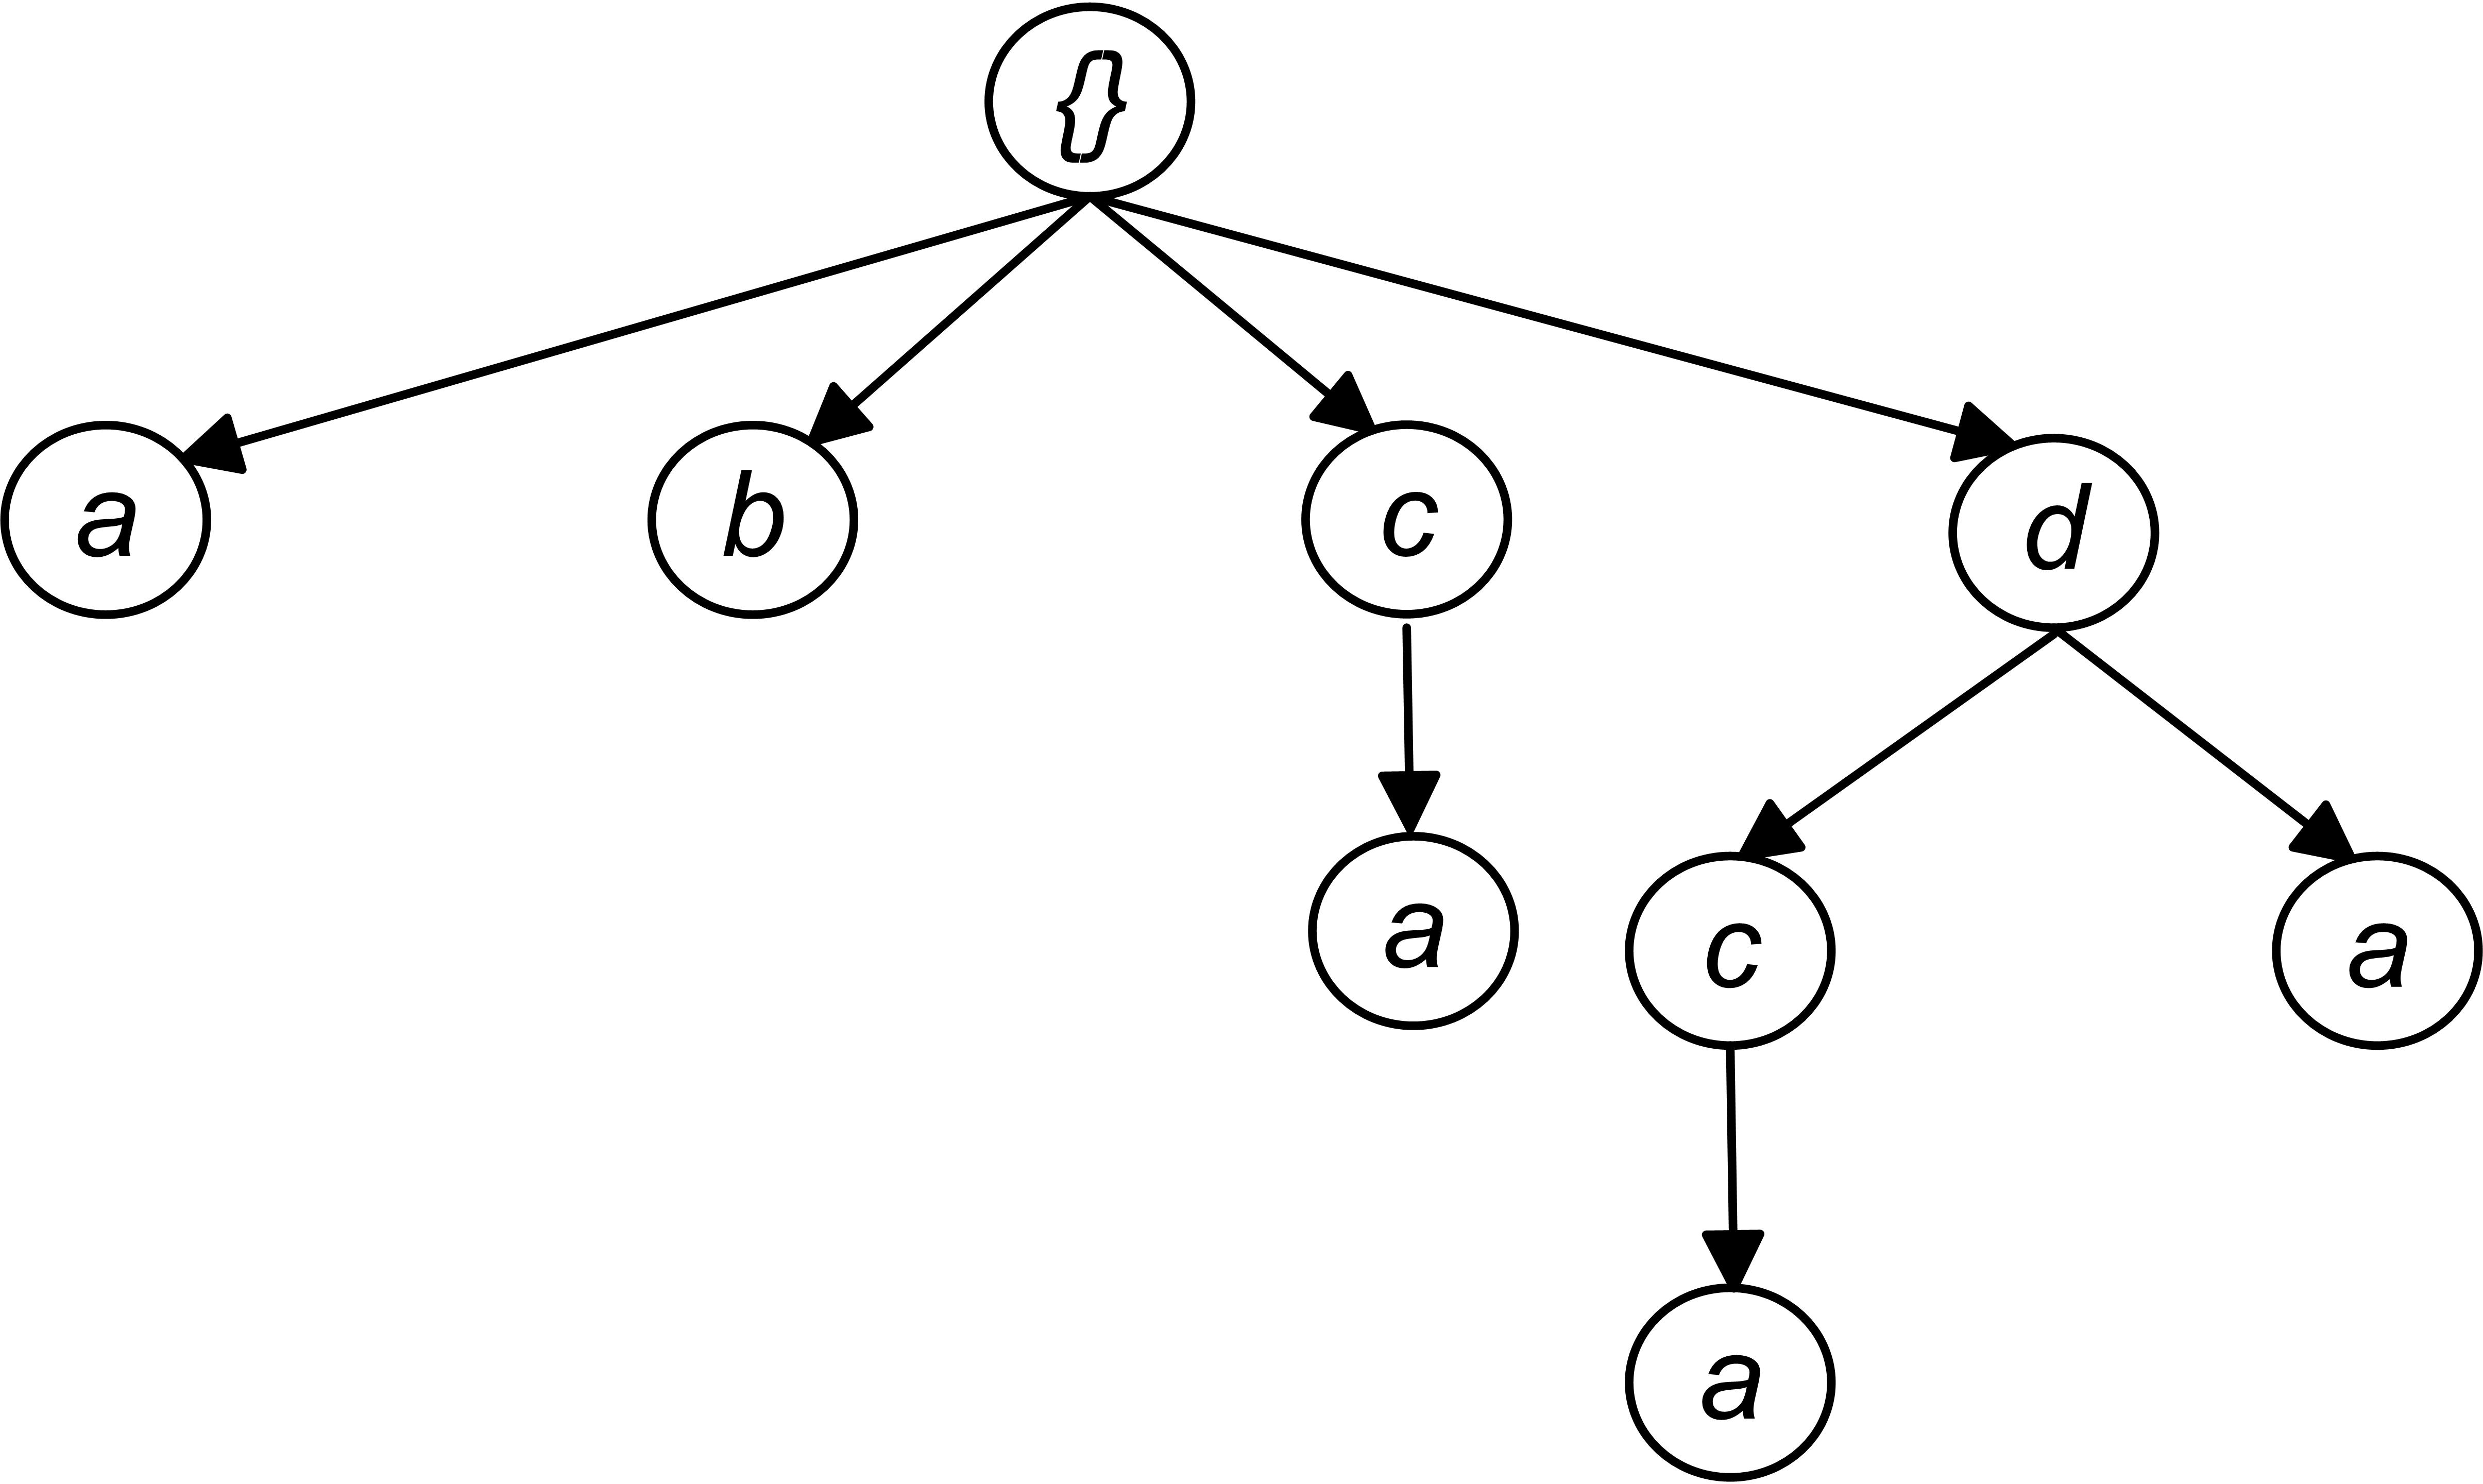
\includegraphics[width=\textwidth]{images/frequent_tree.jpg}
  \captionof{figure}{\emph{Frequent Item Tree} }
\end{minipage}
\caption{Frequent Patterns and Pattern Trees}
\label{figure:frequent_patterns}
\end{figure}
\begin{figure}
\begin{minipage}{.4\textwidth}
  \centering
  
	\begin{center}
	\begin{tabular}{ |c|c| } 
 	\hline
 		No & Items \\ \hline\hline
 		T\textsubscript{1} & \emph{a(0.9),c(0.6),d(0.5)}\\ \hline
 		T\textsubscript{2}& \emph{a(0.9),b(0.4),e(0.1)}\\ \hline
 		T\textsubscript{3}& \emph{a(0.2),c(0.9),d(0.7)}\\ \hline
 		T\textsubscript{4}& \emph{b(0.3),c(0.9)}\\ \hline
 		T\textsubscript{5}& \emph{a(0.1),b(0.3),c(0.9)} \\ \hline
 		T\textsubscript{6} & \emph{a(0.9),e(0.3)
}\\ \hline
\end{tabular}
\end{center}  
\end{minipage}
\hfill
\begin{minipage}{0.50\textwidth}
  \centering
  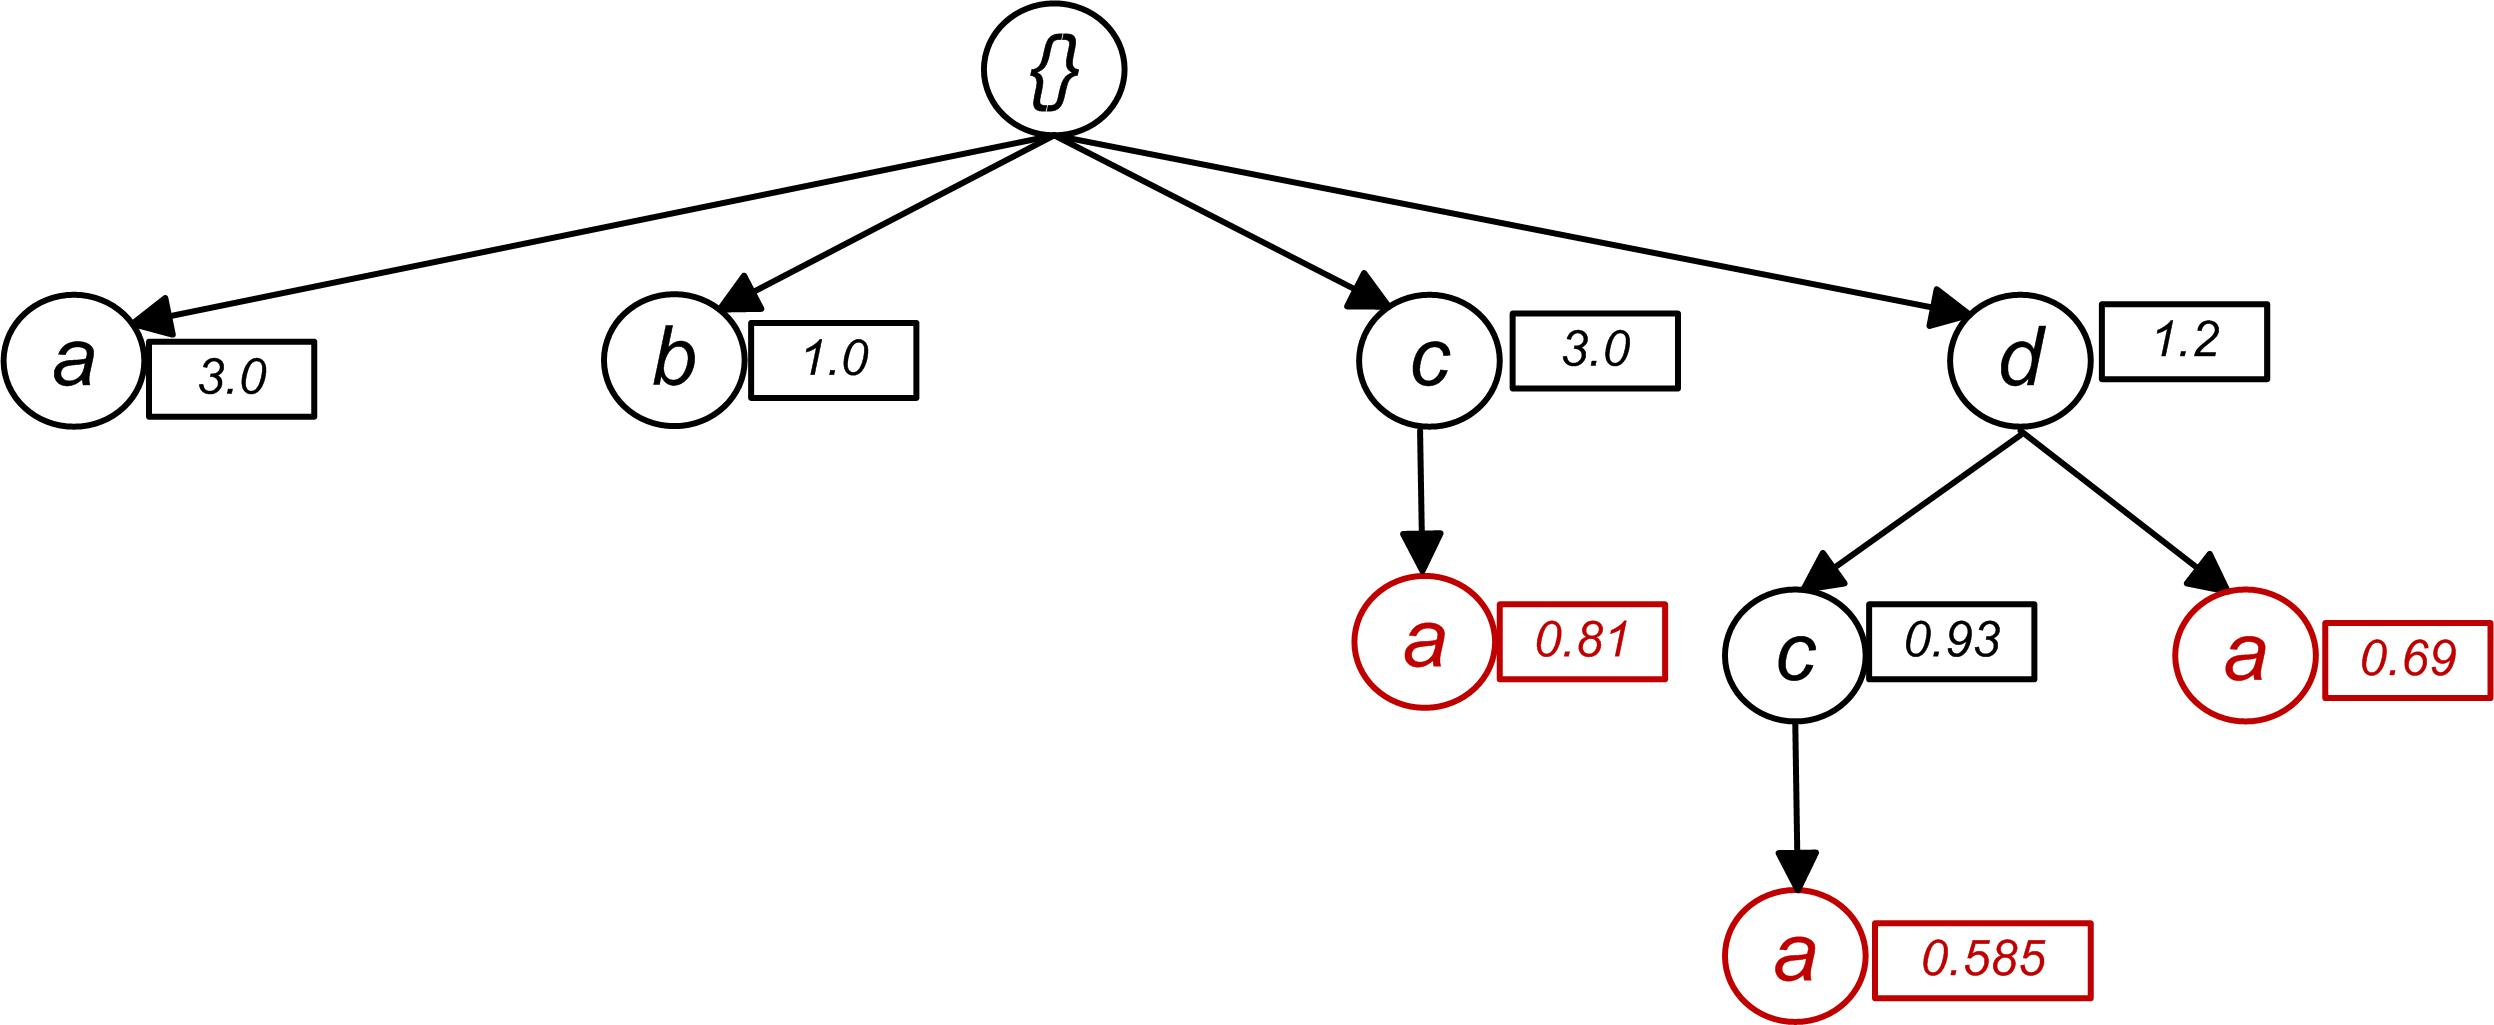
\includegraphics[width=\textwidth]{images/frequent_tree_final.jpg}
\end{minipage}
\caption{Transaction Table and Pattern Trees identifying \emph{False Positives}}
\label{figure:frequent_patterns_final}
\end{figure}
%\end{document}

\clearpage    
    \subsection{Algorithm}
    In this section we have given our proposed algorithms. First we gave algorithm-\ref{algorithm:cap_assignment} that is for I\textsuperscript{cap} calculation for each item of any transaction. Then algorithm-\ref{algorithm:tree_construction} is for \emph{US-tree} construction and algorithm-\ref{algorithm:mine} is for mining with \emph{USFP-growth} algorithm.
    %\documentclass[a4paper]{article}

%\usepackage[english]{babel}
%\usepackage[utf8]{inputenc}
%\usepackage{amsmath}
%\usepackage{amsfonts}
%\usepackage{graphicx}
%\usepackage[colorinlistoftodos]{todonotes}
%\usepackage{algorithm}
%\usepackage{algpseudocode}

%\usepackage{geometry}
% \geometry{
% a4paper,
% total={210mm,297mm},
% left=20mm,
% right=20mm,
% top=20mm,
% bottom=20mm,
% }

%\begin{document}
  \begin{algorithm}
   \caption{\emph{U\textsuperscript{cap}} Assignment}
    \begin{algorithmic}[1]
      \Function{Assign\emph{U\textsuperscript{cap}}}{$Batch$ $B$}
			\For {Transaction $T$  in Batch}
				\For {$\$i=1$ to size of ( $T$ )}
					\State $\$Item$ = T[$[i]$]
					\If{$i=1$}
						\State $\$Item$[\emph{U\textsuperscript{cap}}] $=$ $Probability(\$Item)$
					\Else
						\State $\$Item$[\emph{U\textsuperscript{cap}}] $=$ MAX \{ $Probability(\$T[1])$ to $Probability(\$T[i-1])$ \} $*$ $Probability(\$Item)$
					\EndIf
				\EndFor
			\EndFor
       \EndFunction

\end{algorithmic}
\end{algorithm}
%\end{document}
\clearpage
    \section{Summary}
    In this section, we will discuss our proposed approach for mining frequent pattern over large uncertain stream data. Stream Data has a special property that it comes and flows away. For this reason, we will lose data after data stream has flown away. To resolve this, we will propose a window based approach where we will keep the most recent information in a tree structure as the most recent data is most valuable. Later we will show how the window will slide, remove old data and insert new data in the window. As, for uncertain data stream each same item in the different transaction has different existential probability, it becomes very hard to merge (share) this node in the tree. This uncertainty property of item makes the tree huge. We have proposed a new \emph{U\textsuperscript{cap}} value for each item that helps to share a single node when constructing the tree which we named as \emph{US-tree}. We will show that our proposed tree \emph{US-tree} will be very compact and very efficient for later mining. Later, will describe an approach for mining the \emph {US-tree} named \emph{USFP-growth} which is \emph{FP-growth} like approach. Later we will propose a method for filtering false positive from finding most probable frequent patterns.
%\end{document}
